% UG-MARL project report (ROADMAP 9.1). Build from report/:  latexmk -pdf main.tex
% Tables and \res{..}{..}{..} numbers are generated: python scripts/report_tables.py
\documentclass[10pt,a4paper,oneside]{report}

\usepackage[T1]{fontenc}
\usepackage[utf8]{inputenc}
\usepackage{lmodern}
\usepackage{microtype}
\usepackage[a4paper,margin=2cm]{geometry}
\usepackage{amsmath,amssymb}
\usepackage{graphicx}
\usepackage{booktabs}
\usepackage{array}
\usepackage[font=small,labelfont=bf,skip=4pt]{caption}
\usepackage{subcaption}
\usepackage{algorithm}
\usepackage{algpseudocode}
\usepackage{enumitem}
\usepackage{titlesec}
\usepackage[titles]{tocloft}
\usepackage[numbers,sort&compress]{natbib}
\usepackage{xcolor}
\usepackage[hidelinks]{hyperref}
\usepackage[nameinlink,noabbrev,capitalise]{cleveref}

\graphicspath{{figures/}{../docs/figures/results/}{../docs/figures/eda/}{../docs/figures/training/}}

% compact, numbered chapters that run on without a page break
\titleclass{\chapter}{straight}
\titleformat{\chapter}[hang]{\normalfont\Large\bfseries}{\thechapter}{0.8em}{}
\titlespacing*{\chapter}{0pt}{12pt plus 4pt minus 2pt}{6pt}
\titleformat{\section}{\normalfont\large\bfseries}{\thesection}{0.7em}{}
\titlespacing*{\section}{0pt}{7pt plus 2pt minus 2pt}{2pt}
\titleformat{\subsection}[runin]{\normalfont\normalsize\bfseries}{\thesubsection}{0.6em}{}[.]
\titlespacing*{\subsection}{0pt}{5pt plus 1pt}{0.5em}
\setlist{nosep,leftmargin=1.4em}
\linespread{0.97}
\setlength{\parskip}{2.5pt plus 1pt}
\setlength{\parindent}{0pt}
\setlength{\textfloatsep}{8pt plus 2pt minus 2pt}
\setlength{\floatsep}{6pt plus 2pt minus 2pt}
\setlength{\intextsep}{6pt plus 2pt minus 2pt}
\setlength{\abovedisplayskip}{5pt plus 1pt minus 2pt}
\setlength{\belowdisplayskip}{5pt plus 1pt minus 2pt}
\renewcommand{\topfraction}{0.95}
\renewcommand{\bottomfraction}{0.9}
\renewcommand{\textfraction}{0.05}
\renewcommand{\floatpagefraction}{0.85}
\makeatletter\setlength{\@fptop}{0pt}\makeatother % float pages start at the top
\renewcommand{\bibname}{References}
\setcounter{topnumber}{3}
\setcounter{totalnumber}{4}

% contents, list of figures and list of tables on one page
\setcounter{tocdepth}{1}
\setlength{\cftbeforechapskip}{3pt}
\setlength{\cftbeforetoctitleskip}{0pt}
\setlength{\cftbeforeloftitleskip}{10pt}
\setlength{\cftbeforelottitleskip}{10pt}
\setlength{\cftaftertoctitleskip}{4pt}
\setlength{\cftafterloftitleskip}{4pt}
\setlength{\cftafterlottitleskip}{4pt}
\renewcommand{\cfttoctitlefont}{\Large\bfseries}
\renewcommand{\cftloftitlefont}{\large\bfseries}
\renewcommand{\cftlottitlefont}{\large\bfseries}
\renewcommand{\cftchapfont}{\bfseries\small}
\renewcommand{\cftchappagefont}{\bfseries\small}
\renewcommand{\cftsecfont}{\small}
\renewcommand{\cftsecpagefont}{\small}
\renewcommand{\cftfigfont}{\small}
\renewcommand{\cftfigpagefont}{\small}
\renewcommand{\cfttabfont}{\small}
\renewcommand{\cfttabpagefont}{\small}
\setlength{\cftbeforesecskip}{0pt}
\setlength{\cftbeforefigskip}{0pt}
\setlength{\cftbeforetabskip}{0pt}

\algrenewcommand\algorithmicrequire{\textbf{Input:}}
\algrenewcommand\algorithmicensure{\textbf{Output:}}
\algrenewcommand\algorithmiccomment[1]{\hfill{\footnotesize\textit{#1}}}
\crefname{algorithm}{Algorithm}{Algorithms}
\crefname{equation}{Eq.}{Eqs.}
\crefname{chapter}{Chapter}{Chapters}

\newcommand{\ugmarl}{UG-MARL}
\newcommand{\dt}{\Delta t}
\DeclareMathOperator*{\argmax}{arg\,max}
% Generated by scripts/report_tables.py from docs/results/*.csv -- do not edit.
\makeatletter
\newcommand{\res}[3]{\ifcsname res@#1@#2@#3\endcsname\csname res@#1@#2@#3\endcsname\else\PackageError{report}{unknown result #1/#2/#3}{}\fi}
\@namedef{res@dtt@dqn@clean}{0.0}
\@namedef{res@dtt@dqn@drop0.1}{6.1}
\@namedef{res@dtt@dqn@drop0.2}{12.6}
\@namedef{res@dtt@dqn@noise0.1}{277.6}
\@namedef{res@dtt@dqn@noise0.2}{536.0}
\@namedef{res@dtt@dqn@surge1.5}{80.8}
\@namedef{res@dtt@fixed_time@clean}{0.0}
\@namedef{res@dtt@fixed_time@drop0.1}{0.0}
\@namedef{res@dtt@fixed_time@drop0.2}{0.0}
\@namedef{res@dtt@fixed_time@noise0.1}{0.0}
\@namedef{res@dtt@fixed_time@noise0.2}{0.0}
\@namedef{res@dtt@fixed_time@surge1.5}{199.2}
\@namedef{res@dtt@idqn@clean}{0.0}
\@namedef{res@dtt@idqn@drop0.1}{5.5}
\@namedef{res@dtt@idqn@drop0.2}{14.3}
\@namedef{res@dtt@idqn@noise0.1}{235.4}
\@namedef{res@dtt@idqn@noise0.2}{451.0}
\@namedef{res@dtt@idqn@surge1.5}{147.4}
\@namedef{res@dtt@max_pressure@clean}{0.0}
\@namedef{res@dtt@max_pressure@drop0.1}{-2.9}
\@namedef{res@dtt@max_pressure@drop0.2}{-3.6}
\@namedef{res@dtt@max_pressure@noise0.1}{46.1}
\@namedef{res@dtt@max_pressure@noise0.2}{92.9}
\@namedef{res@dtt@max_pressure@surge1.5}{114.4}
\@namedef{res@dtt@ugmarl-noattn@clean}{0.0}
\@namedef{res@dtt@ugmarl-noattn@drop0.1}{5.2}
\@namedef{res@dtt@ugmarl-noattn@drop0.2}{10.2}
\@namedef{res@dtt@ugmarl-noattn@noise0.1}{75.1}
\@namedef{res@dtt@ugmarl-noattn@noise0.2}{125.1}
\@namedef{res@dtt@ugmarl-noattn@surge1.5}{82.0}
\@namedef{res@dtt@ugmarl-noens@clean}{0.0}
\@namedef{res@dtt@ugmarl-noens@drop0.1}{5.9}
\@namedef{res@dtt@ugmarl-noens@drop0.2}{14.2}
\@namedef{res@dtt@ugmarl-noens@noise0.1}{314.6}
\@namedef{res@dtt@ugmarl-noens@noise0.2}{567.5}
\@namedef{res@dtt@ugmarl-noens@surge1.5}{97.8}
\@namedef{res@dtt@ugmarl-nogate@clean}{0.0}
\@namedef{res@dtt@ugmarl-nogate@drop0.1}{5.1}
\@namedef{res@dtt@ugmarl-nogate@drop0.2}{10.4}
\@namedef{res@dtt@ugmarl-nogate@noise0.1}{302.7}
\@namedef{res@dtt@ugmarl-nogate@noise0.2}{575.2}
\@namedef{res@dtt@ugmarl-nogate@surge1.5}{81.4}
\@namedef{res@dtt@ugmarl@clean}{0.0}
\@namedef{res@dtt@ugmarl@drop0.1}{4.4}
\@namedef{res@dtt@ugmarl@drop0.2}{9.6}
\@namedef{res@dtt@ugmarl@noise0.1}{74.9}
\@namedef{res@dtt@ugmarl@noise0.2}{125.1}
\@namedef{res@dtt@ugmarl@surge1.5}{79.6}
\@namedef{res@fb@dqn@clean}{0}
\@namedef{res@fb@dqn@drop0.1}{0}
\@namedef{res@fb@dqn@drop0.2}{0}
\@namedef{res@fb@dqn@hz-all}{0}
\@namedef{res@fb@dqn@hz-real}{0}
\@namedef{res@fb@dqn@hz-real_5734}{0}
\@namedef{res@fb@dqn@hz-real_5816}{0}
\@namedef{res@fb@dqn@noise0.1}{0}
\@namedef{res@fb@dqn@noise0.2}{0}
\@namedef{res@fb@dqn@surge1.5}{0}
\@namedef{res@fb@fixed_time@clean}{0}
\@namedef{res@fb@fixed_time@drop0.1}{0}
\@namedef{res@fb@fixed_time@drop0.2}{0}
\@namedef{res@fb@fixed_time@hz-all}{0}
\@namedef{res@fb@fixed_time@hz-real}{0}
\@namedef{res@fb@fixed_time@hz-real_5734}{0}
\@namedef{res@fb@fixed_time@hz-real_5816}{0}
\@namedef{res@fb@fixed_time@noise0.1}{0}
\@namedef{res@fb@fixed_time@noise0.2}{0}
\@namedef{res@fb@fixed_time@surge1.5}{0}
\@namedef{res@fb@idqn@clean}{0}
\@namedef{res@fb@idqn@drop0.1}{0}
\@namedef{res@fb@idqn@drop0.2}{0}
\@namedef{res@fb@idqn@noise0.1}{0}
\@namedef{res@fb@idqn@noise0.2}{0}
\@namedef{res@fb@idqn@surge1.5}{0}
\@namedef{res@fb@max_pressure@clean}{0}
\@namedef{res@fb@max_pressure@drop0.1}{0}
\@namedef{res@fb@max_pressure@drop0.2}{0}
\@namedef{res@fb@max_pressure@hz-all}{0}
\@namedef{res@fb@max_pressure@hz-real}{0}
\@namedef{res@fb@max_pressure@hz-real_5734}{0}
\@namedef{res@fb@max_pressure@hz-real_5816}{0}
\@namedef{res@fb@max_pressure@noise0.1}{0}
\@namedef{res@fb@max_pressure@noise0.2}{0}
\@namedef{res@fb@max_pressure@surge1.5}{0}
\@namedef{res@fb@ugmarl-noattn@clean}{21}
\@namedef{res@fb@ugmarl-noattn@drop0.1}{25}
\@namedef{res@fb@ugmarl-noattn@drop0.2}{28}
\@namedef{res@fb@ugmarl-noattn@hz-all}{37}
\@namedef{res@fb@ugmarl-noattn@hz-real}{31}
\@namedef{res@fb@ugmarl-noattn@hz-real_5734}{40}
\@namedef{res@fb@ugmarl-noattn@hz-real_5816}{39}
\@namedef{res@fb@ugmarl-noattn@noise0.1}{84}
\@namedef{res@fb@ugmarl-noattn@noise0.2}{96}
\@namedef{res@fb@ugmarl-noattn@surge1.5}{53}
\@namedef{res@fb@ugmarl-noens@clean}{0}
\@namedef{res@fb@ugmarl-noens@drop0.1}{0}
\@namedef{res@fb@ugmarl-noens@drop0.2}{0}
\@namedef{res@fb@ugmarl-noens@hz-all}{0}
\@namedef{res@fb@ugmarl-noens@hz-real}{0}
\@namedef{res@fb@ugmarl-noens@hz-real_5734}{0}
\@namedef{res@fb@ugmarl-noens@hz-real_5816}{0}
\@namedef{res@fb@ugmarl-noens@noise0.1}{0}
\@namedef{res@fb@ugmarl-noens@noise0.2}{0}
\@namedef{res@fb@ugmarl-noens@surge1.5}{0}
\@namedef{res@fb@ugmarl-nogate@clean}{0}
\@namedef{res@fb@ugmarl-nogate@drop0.1}{0}
\@namedef{res@fb@ugmarl-nogate@drop0.2}{0}
\@namedef{res@fb@ugmarl-nogate@hz-all}{0}
\@namedef{res@fb@ugmarl-nogate@hz-real}{0}
\@namedef{res@fb@ugmarl-nogate@hz-real_5734}{0}
\@namedef{res@fb@ugmarl-nogate@hz-real_5816}{0}
\@namedef{res@fb@ugmarl-nogate@noise0.1}{0}
\@namedef{res@fb@ugmarl-nogate@noise0.2}{0}
\@namedef{res@fb@ugmarl-nogate@surge1.5}{0}
\@namedef{res@fb@ugmarl@clean}{21}
\@namedef{res@fb@ugmarl@drop0.1}{24}
\@namedef{res@fb@ugmarl@drop0.2}{27}
\@namedef{res@fb@ugmarl@hz-all}{34}
\@namedef{res@fb@ugmarl@hz-real}{25}
\@namedef{res@fb@ugmarl@hz-real_5734}{40}
\@namedef{res@fb@ugmarl@hz-real_5816}{37}
\@namedef{res@fb@ugmarl@noise0.1}{83}
\@namedef{res@fb@ugmarl@noise0.2}{96}
\@namedef{res@fb@ugmarl@surge1.5}{55}
\@namedef{res@maxw@dqn@clean}{772}
\@namedef{res@maxw@dqn@drop0.1}{693}
\@namedef{res@maxw@dqn@drop0.2}{621}
\@namedef{res@maxw@dqn@hz-all}{1660}
\@namedef{res@maxw@dqn@hz-real}{877}
\@namedef{res@maxw@dqn@hz-real_5734}{2088}
\@namedef{res@maxw@dqn@hz-real_5816}{2016}
\@namedef{res@maxw@dqn@noise0.1}{2462}
\@namedef{res@maxw@dqn@noise0.2}{3411}
\@namedef{res@maxw@dqn@surge1.5}{1161}
\@namedef{res@maxw@fixed_time@clean}{1417}
\@namedef{res@maxw@fixed_time@drop0.1}{1417}
\@namedef{res@maxw@fixed_time@drop0.2}{1417}
\@namedef{res@maxw@fixed_time@hz-all}{1756}
\@namedef{res@maxw@fixed_time@hz-real}{1396}
\@namedef{res@maxw@fixed_time@hz-real_5734}{2256}
\@namedef{res@maxw@fixed_time@hz-real_5816}{1615}
\@namedef{res@maxw@fixed_time@noise0.1}{1417}
\@namedef{res@maxw@fixed_time@noise0.2}{1417}
\@namedef{res@maxw@fixed_time@surge1.5}{1954}
\@namedef{res@maxw@idqn@clean}{749}
\@namedef{res@maxw@idqn@drop0.1}{775}
\@namedef{res@maxw@idqn@drop0.2}{772}
\@namedef{res@maxw@idqn@noise0.1}{2099}
\@namedef{res@maxw@idqn@noise0.2}{3056}
\@namedef{res@maxw@idqn@surge1.5}{1678}
\@namedef{res@maxw@max_pressure@clean}{1219}
\@namedef{res@maxw@max_pressure@drop0.1}{1212}
\@namedef{res@maxw@max_pressure@drop0.2}{1109}
\@namedef{res@maxw@max_pressure@hz-all}{2734}
\@namedef{res@maxw@max_pressure@hz-real}{1646}
\@namedef{res@maxw@max_pressure@hz-real_5734}{3182}
\@namedef{res@maxw@max_pressure@hz-real_5816}{3373}
\@namedef{res@maxw@max_pressure@noise0.1}{1274}
\@namedef{res@maxw@max_pressure@noise0.2}{1538}
\@namedef{res@maxw@max_pressure@surge1.5}{3260}
\@namedef{res@maxw@ugmarl-noattn@clean}{876}
\@namedef{res@maxw@ugmarl-noattn@drop0.1}{749}
\@namedef{res@maxw@ugmarl-noattn@drop0.2}{666}
\@namedef{res@maxw@ugmarl-noattn@hz-all}{2146}
\@namedef{res@maxw@ugmarl-noattn@hz-real}{889}
\@namedef{res@maxw@ugmarl-noattn@hz-real_5734}{3172}
\@namedef{res@maxw@ugmarl-noattn@hz-real_5816}{2378}
\@namedef{res@maxw@ugmarl-noattn@noise0.1}{1049}
\@namedef{res@maxw@ugmarl-noattn@noise0.2}{1410}
\@namedef{res@maxw@ugmarl-noattn@surge1.5}{2214}
\@namedef{res@maxw@ugmarl-noens@clean}{740}
\@namedef{res@maxw@ugmarl-noens@drop0.1}{697}
\@namedef{res@maxw@ugmarl-noens@drop0.2}{739}
\@namedef{res@maxw@ugmarl-noens@hz-all}{1696}
\@namedef{res@maxw@ugmarl-noens@hz-real}{959}
\@namedef{res@maxw@ugmarl-noens@hz-real_5734}{2040}
\@namedef{res@maxw@ugmarl-noens@hz-real_5816}{2088}
\@namedef{res@maxw@ugmarl-noens@noise0.1}{2449}
\@namedef{res@maxw@ugmarl-noens@noise0.2}{3279}
\@namedef{res@maxw@ugmarl-noens@surge1.5}{1293}
\@namedef{res@maxw@ugmarl-nogate@clean}{910}
\@namedef{res@maxw@ugmarl-nogate@drop0.1}{819}
\@namedef{res@maxw@ugmarl-nogate@drop0.2}{834}
\@namedef{res@maxw@ugmarl-nogate@hz-all}{1939}
\@namedef{res@maxw@ugmarl-nogate@hz-real}{1213}
\@namedef{res@maxw@ugmarl-nogate@hz-real_5734}{2455}
\@namedef{res@maxw@ugmarl-nogate@hz-real_5816}{2148}
\@namedef{res@maxw@ugmarl-nogate@noise0.1}{2409}
\@namedef{res@maxw@ugmarl-nogate@noise0.2}{3306}
\@namedef{res@maxw@ugmarl-nogate@surge1.5}{1430}
\@namedef{res@maxw@ugmarl@clean}{896}
\@namedef{res@maxw@ugmarl@drop0.1}{735}
\@namedef{res@maxw@ugmarl@drop0.2}{789}
\@namedef{res@maxw@ugmarl@hz-all}{2262}
\@namedef{res@maxw@ugmarl@hz-real}{1170}
\@namedef{res@maxw@ugmarl@hz-real_5734}{3167}
\@namedef{res@maxw@ugmarl@hz-real_5816}{2449}
\@namedef{res@maxw@ugmarl@noise0.1}{1212}
\@namedef{res@maxw@ugmarl@noise0.2}{1493}
\@namedef{res@maxw@ugmarl@surge1.5}{2162}
\@namedef{res@pnn@dqn@clean}{301}
\@namedef{res@pnn@dqn@drop0.1}{296}
\@namedef{res@pnn@dqn@drop0.2}{305}
\@namedef{res@pnn@dqn@noise0.1}{1878}
\@namedef{res@pnn@dqn@noise0.2}{3165}
\@namedef{res@pnn@dqn@surge1.5}{617}
\@namedef{res@pnn@fixed_time@clean}{1037}
\@namedef{res@pnn@fixed_time@drop0.1}{1037}
\@namedef{res@pnn@fixed_time@drop0.2}{1037}
\@namedef{res@pnn@fixed_time@noise0.1}{1037}
\@namedef{res@pnn@fixed_time@noise0.2}{1037}
\@namedef{res@pnn@fixed_time@surge1.5}{1369}
\@namedef{res@pnn@idqn@clean}{376}
\@namedef{res@pnn@idqn@drop0.1}{372}
\@namedef{res@pnn@idqn@drop0.2}{384}
\@namedef{res@pnn@idqn@noise0.1}{1545}
\@namedef{res@pnn@idqn@noise0.2}{2545}
\@namedef{res@pnn@idqn@surge1.5}{1158}
\@namedef{res@pnn@max_pressure@clean}{605}
\@namedef{res@pnn@max_pressure@drop0.1}{544}
\@namedef{res@pnn@max_pressure@drop0.2}{481}
\@namedef{res@pnn@max_pressure@noise0.1}{590}
\@namedef{res@pnn@max_pressure@noise0.2}{716}
\@namedef{res@pnn@max_pressure@surge1.5}{1596}
\@namedef{res@pnn@ugmarl-noattn@clean}{327}
\@namedef{res@pnn@ugmarl-noattn@drop0.1}{313}
\@namedef{res@pnn@ugmarl-noattn@drop0.2}{310}
\@namedef{res@pnn@ugmarl-noattn@noise0.1}{529}
\@namedef{res@pnn@ugmarl-noattn@noise0.2}{715}
\@namedef{res@pnn@ugmarl-noattn@surge1.5}{928}
\@namedef{res@pnn@ugmarl-noens@clean}{325}
\@namedef{res@pnn@ugmarl-noens@drop0.1}{333}
\@namedef{res@pnn@ugmarl-noens@drop0.2}{337}
\@namedef{res@pnn@ugmarl-noens@noise0.1}{1836}
\@namedef{res@pnn@ugmarl-noens@noise0.2}{2825}
\@namedef{res@pnn@ugmarl-noens@surge1.5}{817}
\@namedef{res@pnn@ugmarl-nogate@clean}{342}
\@namedef{res@pnn@ugmarl-nogate@drop0.1}{322}
\@namedef{res@pnn@ugmarl-nogate@drop0.2}{326}
\@namedef{res@pnn@ugmarl-nogate@noise0.1}{1935}
\@namedef{res@pnn@ugmarl-nogate@noise0.2}{3012}
\@namedef{res@pnn@ugmarl-nogate@surge1.5}{697}
\@namedef{res@pnn@ugmarl@clean}{346}
\@namedef{res@pnn@ugmarl@drop0.1}{325}
\@namedef{res@pnn@ugmarl@drop0.2}{334}
\@namedef{res@pnn@ugmarl@noise0.1}{549}
\@namedef{res@pnn@ugmarl@noise0.2}{724}
\@namedef{res@pnn@ugmarl@surge1.5}{935}
\@namedef{res@queue@dqn@clean}{0.63}
\@namedef{res@queue@fixed_time@clean}{2.19}
\@namedef{res@queue@idqn@clean}{0.79}
\@namedef{res@queue@max_pressure@clean}{0.95}
\@namedef{res@queue@ugmarl@clean}{0.66}
\@namedef{res@regret@dqn@clean}{0.0}
\@namedef{res@regret@dqn@drop0.1}{0.0}
\@namedef{res@regret@dqn@drop0.2}{0.0}
\@namedef{res@regret@dqn@mean}{102.9}
\@namedef{res@regret@dqn@noise0.1}{202.9}
\@namedef{res@regret@dqn@noise0.2}{414.6}
\@namedef{res@regret@dqn@surge1.5}{0.0}
\@namedef{res@regret@dqn@worst}{414.6}
\@namedef{res@regret@fixed_time@clean}{169.9}
\@namedef{res@regret@fixed_time@drop0.1}{163.9}
\@namedef{res@regret@fixed_time@drop0.2}{157.3}
\@namedef{res@regret@fixed_time@mean}{153.9}
\@namedef{res@regret@fixed_time@noise0.1}{95.3}
\@namedef{res@regret@fixed_time@noise0.2}{48.5}
\@namedef{res@regret@fixed_time@surge1.5}{288.4}
\@namedef{res@regret@fixed_time@worst}{288.4}
\@namedef{res@regret@idqn@clean}{15.7}
\@namedef{res@regret@idqn@drop0.1}{15.1}
\@namedef{res@regret@idqn@drop0.2}{17.4}
\@namedef{res@regret@idqn@mean}{108.7}
\@namedef{res@regret@idqn@noise0.1}{176.5}
\@namedef{res@regret@idqn@noise0.2}{345.2}
\@namedef{res@regret@idqn@surge1.5}{82.3}
\@namedef{res@regret@idqn@worst}{345.2}
\@namedef{res@regret@max_pressure@clean}{28.6}
\@namedef{res@regret@max_pressure@drop0.1}{19.5}
\@namedef{res@regret@max_pressure@drop0.2}{12.4}
\@namedef{res@regret@max_pressure@mean}{20.5}
\@namedef{res@regret@max_pressure@noise0.1}{0.0}
\@namedef{res@regret@max_pressure@noise0.2}{0.0}
\@namedef{res@regret@max_pressure@surge1.5}{62.2}
\@namedef{res@regret@max_pressure@worst}{62.2}
\@namedef{res@regret@ugmarl-noattn@clean}{2.0}
\@namedef{res@regret@ugmarl-noattn@drop0.1}{1.1}
\@namedef{res@regret@ugmarl-noattn@drop0.2}{-0.4}
\@namedef{res@regret@ugmarl-noattn@mean}{2.3}
\@namedef{res@regret@ugmarl-noattn@noise0.1}{2.4}
\@namedef{res@regret@ugmarl-noattn@noise0.2}{5.6}
\@namedef{res@regret@ugmarl-noattn@surge1.5}{3.3}
\@namedef{res@regret@ugmarl-noattn@worst}{5.6}
\@namedef{res@regret@ugmarl-noens@clean}{5.1}
\@namedef{res@regret@ugmarl-noens@drop0.1}{5.0}
\@namedef{res@regret@ugmarl-noens@drop0.2}{6.7}
\@namedef{res@regret@ugmarl-noens@mean}{122.5}
\@namedef{res@regret@ugmarl-noens@noise0.1}{245.1}
\@namedef{res@regret@ugmarl-noens@noise0.2}{451.2}
\@namedef{res@regret@ugmarl-noens@surge1.5}{22.1}
\@namedef{res@regret@ugmarl-noens@worst}{451.2}
\@namedef{res@regret@ugmarl-nogate@clean}{2.8}
\@namedef{res@regret@ugmarl-nogate@drop0.1}{1.8}
\@namedef{res@regret@ugmarl-nogate@drop0.2}{0.6}
\@namedef{res@regret@ugmarl-nogate@mean}{116.0}
\@namedef{res@regret@ugmarl-nogate@noise0.1}{230.9}
\@namedef{res@regret@ugmarl-nogate@noise0.2}{456.6}
\@namedef{res@regret@ugmarl-nogate@surge1.5}{3.4}
\@namedef{res@regret@ugmarl-nogate@worst}{456.6}
\@namedef{res@regret@ugmarl@clean}{3.2}
\@namedef{res@regret@ugmarl@drop0.1}{1.5}
\@namedef{res@regret@ugmarl@drop0.2}{0.2}
\@namedef{res@regret@ugmarl@mean}{2.9}
\@namedef{res@regret@ugmarl@noise0.1}{3.5}
\@namedef{res@regret@ugmarl@noise0.2}{6.8}
\@namedef{res@regret@ugmarl@surge1.5}{2.0}
\@namedef{res@regret@ugmarl@worst}{6.8}
\@namedef{res@thr@dqn@clean}{5007}
\@namedef{res@thr@dqn@drop0.1}{4986}
\@namedef{res@thr@dqn@drop0.2}{4982}
\@namedef{res@thr@dqn@hz-all}{4373}
\@namedef{res@thr@dqn@hz-real}{2721}
\@namedef{res@thr@dqn@hz-real_5734}{5731}
\@namedef{res@thr@dqn@hz-real_5816}{4668}
\@namedef{res@thr@dqn@noise0.1}{4272}
\@namedef{res@thr@dqn@noise0.2}{3375}
\@namedef{res@thr@dqn@surge1.5}{7191}
\@namedef{res@thr@fixed_time@clean}{4617}
\@namedef{res@thr@fixed_time@drop0.1}{4617}
\@namedef{res@thr@fixed_time@drop0.2}{4617}
\@namedef{res@thr@fixed_time@hz-all}{3499}
\@namedef{res@thr@fixed_time@hz-real}{2412}
\@namedef{res@thr@fixed_time@hz-real_5734}{4321}
\@namedef{res@thr@fixed_time@hz-real_5816}{3765}
\@namedef{res@thr@fixed_time@noise0.1}{4617}
\@namedef{res@thr@fixed_time@noise0.2}{4617}
\@namedef{res@thr@fixed_time@surge1.5}{5809}
\@namedef{res@thr@idqn@clean}{4980}
\@namedef{res@thr@idqn@drop0.1}{4966}
\@namedef{res@thr@idqn@drop0.2}{4946}
\@namedef{res@thr@idqn@noise0.1}{4322}
\@namedef{res@thr@idqn@noise0.2}{3632}
\@namedef{res@thr@idqn@surge1.5}{6418}
\@namedef{res@thr@max_pressure@clean}{4950}
\@namedef{res@thr@max_pressure@drop0.1}{4965}
\@namedef{res@thr@max_pressure@drop0.2}{4963}
\@namedef{res@thr@max_pressure@hz-all}{4280}
\@namedef{res@thr@max_pressure@hz-real}{2708}
\@namedef{res@thr@max_pressure@hz-real_5734}{5641}
\@namedef{res@thr@max_pressure@hz-real_5816}{4490}
\@namedef{res@thr@max_pressure@noise0.1}{4882}
\@namedef{res@thr@max_pressure@noise0.2}{4788}
\@namedef{res@thr@max_pressure@surge1.5}{6837}
\@namedef{res@thr@ugmarl-noattn@clean}{4998}
\@namedef{res@thr@ugmarl-noattn@drop0.1}{4994}
\@namedef{res@thr@ugmarl-noattn@drop0.2}{4983}
\@namedef{res@thr@ugmarl-noattn@hz-all}{4390}
\@namedef{res@thr@ugmarl-noattn@hz-real}{2720}
\@namedef{res@thr@ugmarl-noattn@hz-real_5734}{5798}
\@namedef{res@thr@ugmarl-noattn@hz-real_5816}{4652}
\@namedef{res@thr@ugmarl-noattn@noise0.1}{4869}
\@namedef{res@thr@ugmarl-noattn@noise0.2}{4777}
\@namedef{res@thr@ugmarl-noattn@surge1.5}{7169}
\@namedef{res@thr@ugmarl-noens@clean}{4995}
\@namedef{res@thr@ugmarl-noens@drop0.1}{4985}
\@namedef{res@thr@ugmarl-noens@drop0.2}{4972}
\@namedef{res@thr@ugmarl-noens@hz-all}{4322}
\@namedef{res@thr@ugmarl-noens@hz-real}{2709}
\@namedef{res@thr@ugmarl-noens@hz-real_5734}{5710}
\@namedef{res@thr@ugmarl-noens@hz-real_5816}{4545}
\@namedef{res@thr@ugmarl-noens@noise0.1}{4096}
\@namedef{res@thr@ugmarl-noens@noise0.2}{3203}
\@namedef{res@thr@ugmarl-noens@surge1.5}{6987}
\@namedef{res@thr@ugmarl-nogate@clean}{4996}
\@namedef{res@thr@ugmarl-nogate@drop0.1}{4992}
\@namedef{res@thr@ugmarl-nogate@drop0.2}{4978}
\@namedef{res@thr@ugmarl-nogate@hz-all}{4335}
\@namedef{res@thr@ugmarl-nogate@hz-real}{2714}
\@namedef{res@thr@ugmarl-nogate@hz-real_5734}{5706}
\@namedef{res@thr@ugmarl-nogate@hz-real_5816}{4584}
\@namedef{res@thr@ugmarl-nogate@noise0.1}{4164}
\@namedef{res@thr@ugmarl-nogate@noise0.2}{3274}
\@namedef{res@thr@ugmarl-nogate@surge1.5}{7202}
\@namedef{res@thr@ugmarl@clean}{4996}
\@namedef{res@thr@ugmarl@drop0.1}{4994}
\@namedef{res@thr@ugmarl@drop0.2}{4976}
\@namedef{res@thr@ugmarl@hz-all}{4371}
\@namedef{res@thr@ugmarl@hz-real}{2714}
\@namedef{res@thr@ugmarl@hz-real_5734}{5789}
\@namedef{res@thr@ugmarl@hz-real_5816}{4611}
\@namedef{res@thr@ugmarl@noise0.1}{4873}
\@namedef{res@thr@ugmarl@noise0.2}{4776}
\@namedef{res@thr@ugmarl@surge1.5}{7169}
\@namedef{res@tt@dqn@clean}{292.2}
\@namedef{res@tt@dqn@drop0.1}{298.3}
\@namedef{res@tt@dqn@drop0.2}{304.8}
\@namedef{res@tt@dqn@hz-all}{410.4}
\@namedef{res@tt@dqn@hz-real}{343.4}
\@namedef{res@tt@dqn@hz-real_5734}{478.7}
\@namedef{res@tt@dqn@hz-real_5816}{409.1}
\@namedef{res@tt@dqn@noise0.1}{569.8}
\@namedef{res@tt@dqn@noise0.2}{828.2}
\@namedef{res@tt@dqn@surge1.5}{373.0}
\@namedef{res@tt@fixed_time@clean}{462.2}
\@namedef{res@tt@fixed_time@drop0.1}{462.2}
\@namedef{res@tt@fixed_time@drop0.2}{462.2}
\@namedef{res@tt@fixed_time@hz-all}{667.5}
\@namedef{res@tt@fixed_time@hz-real}{590.5}
\@namedef{res@tt@fixed_time@hz-real_5734}{841.7}
\@namedef{res@tt@fixed_time@hz-real_5816}{570.2}
\@namedef{res@tt@fixed_time@noise0.1}{462.2}
\@namedef{res@tt@fixed_time@noise0.2}{462.2}
\@namedef{res@tt@fixed_time@surge1.5}{661.4}
\@namedef{res@tt@idqn@clean}{307.9}
\@namedef{res@tt@idqn@drop0.1}{313.4}
\@namedef{res@tt@idqn@drop0.2}{322.3}
\@namedef{res@tt@idqn@noise0.1}{543.3}
\@namedef{res@tt@idqn@noise0.2}{758.9}
\@namedef{res@tt@idqn@surge1.5}{455.3}
\@namedef{res@tt@max_pressure@clean}{320.8}
\@namedef{res@tt@max_pressure@drop0.1}{317.8}
\@namedef{res@tt@max_pressure@drop0.2}{317.2}
\@namedef{res@tt@max_pressure@hz-all}{431.8}
\@namedef{res@tt@max_pressure@hz-real}{360.7}
\@namedef{res@tt@max_pressure@hz-real_5734}{500.0}
\@namedef{res@tt@max_pressure@hz-real_5816}{434.7}
\@namedef{res@tt@max_pressure@noise0.1}{366.9}
\@namedef{res@tt@max_pressure@noise0.2}{413.7}
\@namedef{res@tt@max_pressure@surge1.5}{435.2}
\@namedef{res@tt@ugmarl-noattn@clean}{294.2}
\@namedef{res@tt@ugmarl-noattn@drop0.1}{299.4}
\@namedef{res@tt@ugmarl-noattn@drop0.2}{304.4}
\@namedef{res@tt@ugmarl-noattn@hz-all}{403.8}
\@namedef{res@tt@ugmarl-noattn@hz-real}{341.5}
\@namedef{res@tt@ugmarl-noattn@hz-real_5734}{460.2}
\@namedef{res@tt@ugmarl-noattn@hz-real_5816}{409.6}
\@namedef{res@tt@ugmarl-noattn@noise0.1}{369.3}
\@namedef{res@tt@ugmarl-noattn@noise0.2}{419.3}
\@namedef{res@tt@ugmarl-noattn@surge1.5}{376.3}
\@namedef{res@tt@ugmarl-noens@clean}{297.3}
\@namedef{res@tt@ugmarl-noens@drop0.1}{303.2}
\@namedef{res@tt@ugmarl-noens@drop0.2}{311.6}
\@namedef{res@tt@ugmarl-noens@hz-all}{423.7}
\@namedef{res@tt@ugmarl-noens@hz-real}{351.7}
\@namedef{res@tt@ugmarl-noens@hz-real_5734}{493.7}
\@namedef{res@tt@ugmarl-noens@hz-real_5816}{425.7}
\@namedef{res@tt@ugmarl-noens@noise0.1}{611.9}
\@namedef{res@tt@ugmarl-noens@noise0.2}{864.9}
\@namedef{res@tt@ugmarl-noens@surge1.5}{395.1}
\@namedef{res@tt@ugmarl-nogate@clean}{295.0}
\@namedef{res@tt@ugmarl-nogate@drop0.1}{300.1}
\@namedef{res@tt@ugmarl-nogate@drop0.2}{305.4}
\@namedef{res@tt@ugmarl-nogate@hz-all}{420.1}
\@namedef{res@tt@ugmarl-nogate@hz-real}{348.9}
\@namedef{res@tt@ugmarl-nogate@hz-real_5734}{491.7}
\@namedef{res@tt@ugmarl-nogate@hz-real_5816}{419.8}
\@namedef{res@tt@ugmarl-nogate@noise0.1}{597.7}
\@namedef{res@tt@ugmarl-nogate@noise0.2}{870.2}
\@namedef{res@tt@ugmarl-nogate@surge1.5}{376.4}
\@namedef{res@tt@ugmarl@clean}{295.4}
\@namedef{res@tt@ugmarl@drop0.1}{299.8}
\@namedef{res@tt@ugmarl@drop0.2}{305.1}
\@namedef{res@tt@ugmarl@hz-all}{410.0}
\@namedef{res@tt@ugmarl@hz-real}{347.3}
\@namedef{res@tt@ugmarl@hz-real_5734}{466.4}
\@namedef{res@tt@ugmarl@hz-real_5816}{416.3}
\@namedef{res@tt@ugmarl@noise0.1}{370.4}
\@namedef{res@tt@ugmarl@noise0.2}{420.5}
\@namedef{res@tt@ugmarl@surge1.5}{375.0}
\@namedef{res@tthi@dqn@clean}{293.0}
\@namedef{res@tthi@dqn@drop0.1}{299.3}
\@namedef{res@tthi@dqn@drop0.2}{306.2}
\@namedef{res@tthi@dqn@noise0.1}{609.6}
\@namedef{res@tthi@dqn@noise0.2}{873.3}
\@namedef{res@tthi@dqn@surge1.5}{378.7}
\@namedef{res@tthi@fixed_time@clean}{462.2}
\@namedef{res@tthi@fixed_time@drop0.1}{462.2}
\@namedef{res@tthi@fixed_time@drop0.2}{462.2}
\@namedef{res@tthi@fixed_time@noise0.1}{462.2}
\@namedef{res@tthi@fixed_time@noise0.2}{462.2}
\@namedef{res@tthi@fixed_time@surge1.5}{666.6}
\@namedef{res@tthi@idqn@clean}{309.7}
\@namedef{res@tthi@idqn@drop0.1}{315.2}
\@namedef{res@tthi@idqn@drop0.2}{323.6}
\@namedef{res@tthi@idqn@noise0.1}{610.7}
\@namedef{res@tthi@idqn@noise0.2}{800.6}
\@namedef{res@tthi@idqn@surge1.5}{544.0}
\@namedef{res@tthi@max_pressure@clean}{320.8}
\@namedef{res@tthi@max_pressure@drop0.1}{318.9}
\@namedef{res@tthi@max_pressure@drop0.2}{319.8}
\@namedef{res@tthi@max_pressure@noise0.1}{369.0}
\@namedef{res@tthi@max_pressure@noise0.2}{418.6}
\@namedef{res@tthi@max_pressure@surge1.5}{440.5}
\@namedef{res@tthi@ugmarl-noattn@clean}{295.5}
\@namedef{res@tthi@ugmarl-noattn@drop0.1}{301.3}
\@namedef{res@tthi@ugmarl-noattn@drop0.2}{306.4}
\@namedef{res@tthi@ugmarl-noattn@noise0.1}{373.4}
\@namedef{res@tthi@ugmarl-noattn@noise0.2}{423.2}
\@namedef{res@tthi@ugmarl-noattn@surge1.5}{379.7}
\@namedef{res@tthi@ugmarl-noens@clean}{299.2}
\@namedef{res@tthi@ugmarl-noens@drop0.1}{306.8}
\@namedef{res@tthi@ugmarl-noens@drop0.2}{318.2}
\@namedef{res@tthi@ugmarl-noens@noise0.1}{648.8}
\@namedef{res@tthi@ugmarl-noens@noise0.2}{1032.2}
\@namedef{res@tthi@ugmarl-noens@surge1.5}{444.9}
\@namedef{res@tthi@ugmarl-nogate@clean}{296.3}
\@namedef{res@tthi@ugmarl-nogate@drop0.1}{302.9}
\@namedef{res@tthi@ugmarl-nogate@drop0.2}{311.2}
\@namedef{res@tthi@ugmarl-nogate@noise0.1}{664.1}
\@namedef{res@tthi@ugmarl-nogate@noise0.2}{926.0}
\@namedef{res@tthi@ugmarl-nogate@surge1.5}{383.0}
\@namedef{res@tthi@ugmarl@clean}{296.8}
\@namedef{res@tthi@ugmarl@drop0.1}{302.0}
\@namedef{res@tthi@ugmarl@drop0.2}{309.0}
\@namedef{res@tthi@ugmarl@noise0.1}{378.8}
\@namedef{res@tthi@ugmarl@noise0.2}{429.6}
\@namedef{res@tthi@ugmarl@surge1.5}{381.0}
\@namedef{res@ttlo@dqn@clean}{291.4}
\@namedef{res@ttlo@dqn@drop0.1}{297.3}
\@namedef{res@ttlo@dqn@drop0.2}{303.4}
\@namedef{res@ttlo@dqn@noise0.1}{530.0}
\@namedef{res@ttlo@dqn@noise0.2}{783.1}
\@namedef{res@ttlo@dqn@surge1.5}{367.3}
\@namedef{res@ttlo@fixed_time@clean}{462.2}
\@namedef{res@ttlo@fixed_time@drop0.1}{462.2}
\@namedef{res@ttlo@fixed_time@drop0.2}{462.2}
\@namedef{res@ttlo@fixed_time@noise0.1}{462.2}
\@namedef{res@ttlo@fixed_time@noise0.2}{462.2}
\@namedef{res@ttlo@fixed_time@surge1.5}{656.1}
\@namedef{res@ttlo@idqn@clean}{306.1}
\@namedef{res@ttlo@idqn@drop0.1}{311.6}
\@namedef{res@ttlo@idqn@drop0.2}{320.9}
\@namedef{res@ttlo@idqn@noise0.1}{476.0}
\@namedef{res@ttlo@idqn@noise0.2}{717.2}
\@namedef{res@ttlo@idqn@surge1.5}{366.6}
\@namedef{res@ttlo@max_pressure@clean}{320.8}
\@namedef{res@ttlo@max_pressure@drop0.1}{316.8}
\@namedef{res@ttlo@max_pressure@drop0.2}{314.6}
\@namedef{res@ttlo@max_pressure@noise0.1}{364.7}
\@namedef{res@ttlo@max_pressure@noise0.2}{408.7}
\@namedef{res@ttlo@max_pressure@surge1.5}{429.8}
\@namedef{res@ttlo@ugmarl-noattn@clean}{292.9}
\@namedef{res@ttlo@ugmarl-noattn@drop0.1}{297.4}
\@namedef{res@ttlo@ugmarl-noattn@drop0.2}{302.4}
\@namedef{res@ttlo@ugmarl-noattn@noise0.1}{365.2}
\@namedef{res@ttlo@ugmarl-noattn@noise0.2}{415.3}
\@namedef{res@ttlo@ugmarl-noattn@surge1.5}{372.8}
\@namedef{res@ttlo@ugmarl-noens@clean}{295.4}
\@namedef{res@ttlo@ugmarl-noens@drop0.1}{299.7}
\@namedef{res@ttlo@ugmarl-noens@drop0.2}{305.0}
\@namedef{res@ttlo@ugmarl-noens@noise0.1}{575.1}
\@namedef{res@ttlo@ugmarl-noens@noise0.2}{697.5}
\@namedef{res@ttlo@ugmarl-noens@surge1.5}{345.2}
\@namedef{res@ttlo@ugmarl-nogate@clean}{293.7}
\@namedef{res@ttlo@ugmarl-nogate@drop0.1}{297.2}
\@namedef{res@ttlo@ugmarl-nogate@drop0.2}{299.6}
\@namedef{res@ttlo@ugmarl-nogate@noise0.1}{531.3}
\@namedef{res@ttlo@ugmarl-nogate@noise0.2}{814.4}
\@namedef{res@ttlo@ugmarl-nogate@surge1.5}{369.7}
\@namedef{res@ttlo@ugmarl@clean}{294.1}
\@namedef{res@ttlo@ugmarl@drop0.1}{297.6}
\@namedef{res@ttlo@ugmarl@drop0.2}{301.1}
\@namedef{res@ttlo@ugmarl@noise0.1}{362.0}
\@namedef{res@ttlo@ugmarl@noise0.2}{411.3}
\@namedef{res@ttlo@ugmarl@surge1.5}{368.9}
\@namedef{res@ttsd@dqn@clean}{0.6}
\@namedef{res@ttsd@dqn@drop0.1}{0.8}
\@namedef{res@ttsd@dqn@drop0.2}{1.1}
\@namedef{res@ttsd@dqn@hz-all}{7.1}
\@namedef{res@ttsd@dqn@hz-real}{2.1}
\@namedef{res@ttsd@dqn@hz-real_5734}{22.7}
\@namedef{res@ttsd@dqn@hz-real_5816}{4.9}
\@namedef{res@ttsd@dqn@noise0.1}{32.0}
\@namedef{res@ttsd@dqn@noise0.2}{36.3}
\@namedef{res@ttsd@dqn@surge1.5}{4.6}
\@namedef{res@ttsd@fixed_time@clean}{0.0}
\@namedef{res@ttsd@fixed_time@drop0.1}{0.0}
\@namedef{res@ttsd@fixed_time@drop0.2}{0.0}
\@namedef{res@ttsd@fixed_time@hz-all}{0.0}
\@namedef{res@ttsd@fixed_time@hz-real}{0.0}
\@namedef{res@ttsd@fixed_time@hz-real_5734}{0.0}
\@namedef{res@ttsd@fixed_time@hz-real_5816}{0.0}
\@namedef{res@ttsd@fixed_time@noise0.1}{0.0}
\@namedef{res@ttsd@fixed_time@noise0.2}{0.0}
\@namedef{res@ttsd@fixed_time@surge1.5}{4.2}
\@namedef{res@ttsd@idqn@clean}{1.4}
\@namedef{res@ttsd@idqn@drop0.1}{1.4}
\@namedef{res@ttsd@idqn@drop0.2}{1.1}
\@namedef{res@ttsd@idqn@noise0.1}{54.2}
\@namedef{res@ttsd@idqn@noise0.2}{33.6}
\@namedef{res@ttsd@idqn@surge1.5}{71.5}
\@namedef{res@ttsd@max_pressure@clean}{0.0}
\@namedef{res@ttsd@max_pressure@drop0.1}{0.8}
\@namedef{res@ttsd@max_pressure@drop0.2}{2.1}
\@namedef{res@ttsd@max_pressure@hz-all}{0.0}
\@namedef{res@ttsd@max_pressure@hz-real}{0.0}
\@namedef{res@ttsd@max_pressure@hz-real_5734}{0.0}
\@namedef{res@ttsd@max_pressure@hz-real_5816}{0.0}
\@namedef{res@ttsd@max_pressure@noise0.1}{1.7}
\@namedef{res@ttsd@max_pressure@noise0.2}{4.0}
\@namedef{res@ttsd@max_pressure@surge1.5}{4.3}
\@namedef{res@ttsd@ugmarl-noattn@clean}{1.1}
\@namedef{res@ttsd@ugmarl-noattn@drop0.1}{1.6}
\@namedef{res@ttsd@ugmarl-noattn@drop0.2}{1.6}
\@namedef{res@ttsd@ugmarl-noattn@hz-all}{1.2}
\@namedef{res@ttsd@ugmarl-noattn@hz-real}{0.7}
\@namedef{res@ttsd@ugmarl-noattn@hz-real_5734}{5.1}
\@namedef{res@ttsd@ugmarl-noattn@hz-real_5816}{1.9}
\@namedef{res@ttsd@ugmarl-noattn@noise0.1}{3.3}
\@namedef{res@ttsd@ugmarl-noattn@noise0.2}{3.1}
\@namedef{res@ttsd@ugmarl-noattn@surge1.5}{2.8}
\@namedef{res@ttsd@ugmarl-noens@clean}{1.5}
\@namedef{res@ttsd@ugmarl-noens@drop0.1}{2.8}
\@namedef{res@ttsd@ugmarl-noens@drop0.2}{5.3}
\@namedef{res@ttsd@ugmarl-noens@hz-all}{14.9}
\@namedef{res@ttsd@ugmarl-noens@hz-real}{2.9}
\@namedef{res@ttsd@ugmarl-noens@hz-real_5734}{39.2}
\@namedef{res@ttsd@ugmarl-noens@hz-real_5816}{8.9}
\@namedef{res@ttsd@ugmarl-noens@noise0.1}{29.7}
\@namedef{res@ttsd@ugmarl-noens@noise0.2}{134.8}
\@namedef{res@ttsd@ugmarl-noens@surge1.5}{40.1}
\@namedef{res@ttsd@ugmarl-nogate@clean}{1.0}
\@namedef{res@ttsd@ugmarl-nogate@drop0.1}{2.3}
\@namedef{res@ttsd@ugmarl-nogate@drop0.2}{4.6}
\@namedef{res@ttsd@ugmarl-nogate@hz-all}{14.6}
\@namedef{res@ttsd@ugmarl-nogate@hz-real}{4.3}
\@namedef{res@ttsd@ugmarl-nogate@hz-real_5734}{35.6}
\@namedef{res@ttsd@ugmarl-nogate@hz-real_5816}{10.1}
\@namedef{res@ttsd@ugmarl-nogate@noise0.1}{53.5}
\@namedef{res@ttsd@ugmarl-nogate@noise0.2}{45.0}
\@namedef{res@ttsd@ugmarl-nogate@surge1.5}{5.4}
\@namedef{res@ttsd@ugmarl@clean}{1.1}
\@namedef{res@ttsd@ugmarl@drop0.1}{1.8}
\@namedef{res@ttsd@ugmarl@drop0.2}{3.2}
\@namedef{res@ttsd@ugmarl@hz-all}{2.9}
\@namedef{res@ttsd@ugmarl@hz-real}{3.5}
\@namedef{res@ttsd@ugmarl@hz-real_5734}{8.5}
\@namedef{res@ttsd@ugmarl@hz-real_5816}{2.6}
\@namedef{res@ttsd@ugmarl@noise0.1}{6.8}
\@namedef{res@ttsd@ugmarl@noise0.2}{7.4}
\@namedef{res@ttsd@ugmarl@surge1.5}{4.9}
\@namedef{res@wait@dqn@clean}{57.0}
\@namedef{res@wait@dqn@drop0.1}{62.7}
\@namedef{res@wait@dqn@drop0.2}{68.8}
\@namedef{res@wait@dqn@noise0.1}{273.4}
\@namedef{res@wait@dqn@noise0.2}{500.9}
\@namedef{res@wait@dqn@surge1.5}{117.7}
\@namedef{res@wait@fixed_time@clean}{210.1}
\@namedef{res@wait@fixed_time@drop0.1}{210.1}
\@namedef{res@wait@fixed_time@drop0.2}{210.1}
\@namedef{res@wait@fixed_time@noise0.1}{210.1}
\@namedef{res@wait@fixed_time@noise0.2}{210.1}
\@namedef{res@wait@fixed_time@surge1.5}{341.9}
\@namedef{res@wait@idqn@clean}{72.3}
\@namedef{res@wait@idqn@drop0.1}{77.4}
\@namedef{res@wait@idqn@drop0.2}{85.6}
\@namedef{res@wait@idqn@noise0.1}{279.1}
\@namedef{res@wait@idqn@noise0.2}{455.1}
\@namedef{res@wait@idqn@surge1.5}{211.1}
\@namedef{res@wait@max_pressure@clean}{87.9}
\@namedef{res@wait@max_pressure@drop0.1}{84.1}
\@namedef{res@wait@max_pressure@drop0.2}{82.8}
\@namedef{res@wait@max_pressure@noise0.1}{130.1}
\@namedef{res@wait@max_pressure@noise0.2}{174.7}
\@namedef{res@wait@max_pressure@surge1.5}{204.0}
\@namedef{res@wait@ugmarl-noattn@clean}{59.2}
\@namedef{res@wait@ugmarl-noattn@drop0.1}{64.0}
\@namedef{res@wait@ugmarl-noattn@drop0.2}{68.8}
\@namedef{res@wait@ugmarl-noattn@noise0.1}{131.9}
\@namedef{res@wait@ugmarl-noattn@noise0.2}{180.2}
\@namedef{res@wait@ugmarl-noattn@surge1.5}{136.3}
\@namedef{res@wait@ugmarl-noens@clean}{62.0}
\@namedef{res@wait@ugmarl-noens@drop0.1}{67.5}
\@namedef{res@wait@ugmarl-noens@drop0.2}{75.0}
\@namedef{res@wait@ugmarl-noens@noise0.1}{341.2}
\@namedef{res@wait@ugmarl-noens@noise0.2}{575.7}
\@namedef{res@wait@ugmarl-noens@surge1.5}{151.2}
\@namedef{res@wait@ugmarl-nogate@clean}{60.0}
\@namedef{res@wait@ugmarl-nogate@drop0.1}{64.5}
\@namedef{res@wait@ugmarl-nogate@drop0.2}{69.4}
\@namedef{res@wait@ugmarl-nogate@noise0.1}{314.4}
\@namedef{res@wait@ugmarl-nogate@noise0.2}{553.9}
\@namedef{res@wait@ugmarl-nogate@surge1.5}{126.1}
\@namedef{res@wait@ugmarl@clean}{60.5}
\@namedef{res@wait@ugmarl@drop0.1}{64.4}
\@namedef{res@wait@ugmarl@drop0.2}{69.5}
\@namedef{res@wait@ugmarl@noise0.1}{132.6}
\@namedef{res@wait@ugmarl@noise0.2}{180.8}
\@namedef{res@wait@ugmarl@surge1.5}{135.3}
\makeatother

\newcommand{\posterlink}{\url{https://canva.link/nj4h08y8a6coxa5}}

\begin{document}

% ---------------- title block (no separate title page) ----------------
\begin{center}
{\small Machine Learning Project Report \quad$\cdot$\quad Problem Statement 16: Agentic Artificial Intelligence\par}
\vspace{6pt}
{\LARGE\bfseries Uncertainty-Gated Multi-Agent Reinforcement Learning\\[2pt]
for Adaptive Traffic Signal Control\par}
\vspace{8pt}
{\large Manda Saad\par}
\vspace{2pt}
{\small Roll No.\ 2401AI28 \quad$\cdot$\quad manda\_2401ai28@iitp.ac.in\par}
{\small Computer Science and Engineering, Indian Institute of Technology Patna \quad$\cdot$\quad November 2026\par}
\end{center}
\vspace{4pt}
\hrule
\vspace{6pt}

\chapter*{Abstract}
\addcontentsline{toc}{chapter}{Abstract}

Reinforcement-learning (RL) controllers for traffic signals cut average travel time, but they
cannot tell when one of their decisions is unreliable, and they break down when detector
readings differ from what they saw in training. Max-Pressure, a rule-based controller, keeps
queues stable under known assumptions but cannot learn. This project compares a conventional
controller (Fixed-Time, Max-Pressure), a single-agent RL controller (one DQN shared by all
intersections) and a multi-agent one (independent DQN, IDQN) on real traffic from Jinan
(12 intersections) and Hangzhou (16 intersections) in the CityFlow simulator, and proposes
\ugmarl{} (Uncertainty-Gated Multi-Agent Reinforcement Learning). Every intersection is an
agent of one shared network that attends to its neighbours and ends in three Q-value heads. When
the heads disagree by more than a threshold chosen on validation data, the decision goes to
Max-Pressure instead. All design choices used training and validation flows only; the test
flow and the second city were simulated once, with five seeds. On the Jinan test flow
\ugmarl{} reaches an average travel time of
$\res{tt}{ugmarl}{clean}\pm\res{ttsd}{ugmarl}{clean}$\,s, ahead of Max-Pressure
(\res{tt}{max_pressure}{clean}\,s) and IDQN (\res{tt}{idqn}{clean}\,s) and
\res{regret}{ugmarl}{clean}\,s behind the shared DQN. With noisy detectors the learned
baselines climb to \res{tt}{idqn}{noise0.2}--\res{tt}{dqn}{noise0.2}\,s while \ugmarl{} stays
at \res{tt}{ugmarl}{noise0.2}\,s, level with Max-Pressure, so across six test conditions its
largest gap to the best controller is \res{regret}{ugmarl}{worst}\,s, against
\res{regret}{max_pressure}{worst}--\res{regret}{dqn}{worst}\,s for the baselines. Neighbour
attention brought no gain, and under a demand surge the fallback lengthens the longest wait
of a single vehicle.

\medskip
\noindent\textbf{Keywords:} traffic signal control, multi-agent reinforcement learning,
epistemic uncertainty, Q-ensemble, Max-Pressure, safe fallback, CityFlow.


% contents and lists follow the abstract directly; chapters run on without page breaks
\begingroup
\let\clearpage\relax
\let\cleardoublepage\relax
\tableofcontents
\vspace{8pt}
\listoffigures
\vspace{8pt}
\listoftables
\endgroup
\vspace{6pt}
\hrule

\chapter{Introduction}
\label{ch:intro}

\section{Background and Motivation}

An agentic AI system observes its environment, decides and acts towards a goal with little
human help. Traffic signal control fits that description closely. Every few seconds each
intersection has to choose which movements get green, using only its own detector readings,
and what one intersection does changes the traffic arriving at its neighbours. Most signals
on real roads still run fixed timing plans or simple actuated rules.

Adaptive controllers come in two families. Rule-based control such as Max-Pressure
\citep{varaiya2013max} needs no training and keeps queues bounded under stated assumptions,
but it never learns from experience. Reinforcement learning (RL) makes each intersection an
agent that learns in simulation, and on the standard benchmarks it gives lower travel times
\citep{wei2019presslight,wei2019colight}. Learned controllers also have the weaknesses that
the problem statement lists for agentic systems. Their decisions become unreliable when the
inputs drift away from the training data, they give no warning when that happens, nothing
bounds their worst case, and their decisions are hard to explain. Benchmark studies add that
reported gains are fragile and that a well-tuned independent DQN often matches newer methods
\citep{ault2021reinforcement}. This project combines the two families. A learned multi-agent
controller picks the phase, and when its own uncertainty about a decision is high, Max-Pressure
picks it instead.

\section{Problem Statement}

Problem Statement 16 asks for a study of the limits of conventional, single-agent and
multi-agent agentic frameworks on a real-world application, and for an improved system with
mathematical justification and experimental validation. Here the problem is:
\emph{given} the queue lengths, vehicle counts and current signal phase at every
intersection of a real road network (Jinan, $3\times4$; held-out city Hangzhou,
$4\times4$), \emph{choose} the next signal phase of each intersection every
$\dt$ seconds over a one-hour episode, \emph{under} minimum-green and yellow-transition
constraints and with possibly noisy or missing detector readings, \emph{so that} the
average travel time is lower than that of the baselines and the longest wait of a vehicle
stays bounded. Each action changes the inputs that follow, which makes this a sequential
decision problem.

\section{Objectives}

\begin{enumerate}
\item Compare conventional (Fixed-Time, Max-Pressure), single-agent RL (a shared DQN) and
multi-agent RL (independent DQN, IDQN) controllers on identical flows and expose their limits.
\item Design \ugmarl{}, with neighbour attention, an ensemble estimate of epistemic
uncertainty and a fallback to Max-Pressure triggered by that uncertainty, and state it
mathematically.
\item Test three hypotheses whose decision rules were fixed before the experiments:
\begin{itemize}
\item \textbf{H1 (performance):} \ugmarl{} has a lower average travel time than IDQN and
Max-Pressure on the test flow, with non-overlapping 95\,\% confidence intervals.
\item \textbf{H2 (safety):} the gate lowers the worst case (maximum per-vehicle wait, loss
of performance under detector noise) compared with the same model without the gate.
\item \textbf{H3 (coordination):} neighbour attention lowers the average travel time
compared with the same model without attention.
\end{itemize}
\item Measure robustness (detector noise, dropout, demand surge), transfer to an unseen
city, cost and explainability. The minimum acceptable outcome is a maximum wait no worse
than that of Max-Pressure.
\end{enumerate}

\section{Scope of the Work}

The work covers two grid networks with real demand, simulated in CityFlow
\citep{zhang2019cityflow} over one-hour episodes. It includes a data audit, an evaluation
protocol frozen before training, four baselines, the proposed model with three ablations,
robustness and cross-city tests, and an error analysis. Real deployment, pedestrians, public
transport, irregular networks and agents built on language models are out of scope.

\section{Contributions}

The contributions are listed in the order in which the work was done.
\begin{enumerate}
\item \textbf{Problem formulation and data design.} Signal control on a road network is
formulated as a decentralised semi-Markov decision problem with minimum-green and transition
constraints, and noisy or missing detector readings are treated as part of that problem
(\cref{sec:arch}). The conventional, single-agent and multi-agent frameworks are compared on
identical flows to measure their limits: the learned baselines beat Max-Pressure by
13--29\,s on clean data and lose to it by 345--415\,s at detector noise 0.2
(\cref{sec:comparison}). The 44 observed values are scaled by lane capacity, so no statistic
is fitted on data, and whole flow files are assigned to the splits before any other step
(\cref{sec:prep}).
\item \textbf{Mathematical modelling and theoretical analysis.} The reward, the learning
target that discounts by elapsed time, the masked ensemble loss, the uncertainty $\sigma$ and
the gate rule with its percentile threshold are written in closed form
(\cref{eq:reward,eq:target,eq:loss,eq:sigma,eq:gate}). The stability claim covers one case only.
When the gate always fires, the controller is Max-Pressure, and the queue-stability theorem of
\citet{varaiya2013max} applies under its assumptions. For the mixed policy a drift argument
is sketched without proof, and its worst case is measured instead (\cref{sec:safety}).
\item \textbf{Proposed framework.} \ugmarl{} is a multi-agent Q-learner. At every
intersection and every decision, the disagreement of an ensemble of Q-heads decides whether
the learned phase or the Max-Pressure phase is applied. Earlier ensemble Q-learners for
signals use the heads only to explore during training \citep{tan2020multiagent}, while
\ugmarl{} keeps them at execution time to choose the action. How it differs from the two
closest methods, Com-MP and the ensemble switch of Hoel et al., is set out in
\cref{sec:gaps}.
\item \textbf{Technical advancement: robustness and interpretability.} With the same weights,
the gate limits the rise in travel time at detector noise 0.2 to
\res{dtt}{ugmarl}{noise0.2}\,s, against \res{dtt}{ugmarl-nogate}{noise0.2}\,s without it.
Over six test conditions the largest regret of \ugmarl{} is \res{regret}{ugmarl}{worst}\,s,
the smallest of all controllers (\cref{tab:robust}). Each decision is logged with $\sigma$,
the gate outcome and the attention weights. CoLight \citep{wei2019colight} presents its
attention weights as an explanation. Here the weights were tested before being read that way:
they rank neighbour influence correctly, but a neighbour carries only about a seventh of the influence
of the intersection's own observation (\cref{sec:discussion}). One joint decision takes
0.81\,ms.
\item \textbf{Experimental validation and comparative analysis.} Four baselines and three
ablations run on real demand under one protocol, frozen before training, with five seeds,
95\,\% confidence intervals, a threshold sensitivity sweep and an error analysis
(\cref{ch:results}). The rules for judging the hypotheses were written before the test flow
was opened. H1 and H2 are supported; H3 is not.
\item \textbf{Generalisation and practical applicability.} The Jinan models are evaluated on
Hangzhou, a city with a different grid size, without retraining or recalibration. There
\ugmarl{} reaches \res{tt}{ugmarl}{hz-all}\,s, level with DQN and 22\,s ahead of Max-Pressure
(\cref{tab:heldout}). Detector noise, dropout and a demand surge stand in for conditions a
deployed controller would meet, and they also show a limit: under the surge the gate makes
the longest wait of a vehicle longer (\cref{sec:discussion}).
\end{enumerate}

\chapter{Literature Review}
\label{ch:literature}

\section{Existing Approaches}

\subsection{Conventional control}
Fixed-time plans set the cycle length and green splits from historical flows, and actuated
systems extend or end a green phase from detector calls with hand-written rules.
Max-Pressure \citep{varaiya2013max} gives green, at each intersection, to the phase with the
largest difference between upstream and downstream queues. It needs only local measurements,
and it keeps the queues of the whole network stable whenever demand lies inside the capacity
region, in a model with unlimited lane storage and known turning ratios. Rule controllers
are transparent and need no training, but the rule never changes. The stability result has
two limits that matter for this project: it is about mean queue lengths, not the wait of a
single vehicle, and its model has neither finite lanes nor time lost at phase changes.

\subsection{Single-agent reinforcement learning}
Deep Q-networks (DQN) \citep{mnih2015human} learn the value of each action from a state
vector and were soon applied to isolated intersections. A single agent either controls one
intersection or treats every intersection on its own with shared weights, which is the
single-agent baseline used here. These agents output a phase and nothing about how far that
choice can be trusted.

\subsection{Multi-agent reinforcement learning}
The simplest multi-agent form gives every intersection its own independent learner (IDQN),
although each agent then faces an environment that changes as the others learn. PressLight
\citep{wei2019presslight} uses the negative pressure as the reward, which ties the learned
objective to Max-Pressure. CoLight \citep{wei2019colight} adds graph attention over the
neighbouring intersections and released the Jinan and Hangzhou flows used in this project.
The gains reported for newer methods are fragile: in a large benchmark a well-tuned
independent DQN matched most of them \citep{ault2021reinforcement}. Two habits limit what
published numbers show. Studies differ in decision interval, transition time and flow files,
so their travel times cannot be compared directly, and evaluation is usually done with perfect
detectors on the demand the agent was trained for, often without reporting the spread
between training runs. Most recent work uses the CityFlow simulator
\citep{zhang2019cityflow}, as this project does.

\subsection{Uncertainty and safe reinforcement learning}
Epistemic uncertainty comes from limited training data, unlike the randomness of the traffic
itself, and an ensemble of independently initialised networks is a simple way to estimate it.
Bootstrapped DQN \citep{osband2016deep} trains several Q-heads on one shared network and
gives each head a random subset of the experience. In signal control, ensembles like this
have been used to explore during training \citep{tan2020multiagent}, not to judge a decision
once the controller is running. In automated driving, by contrast, Hoel et al.\
\citep{hoel2020tactical} let an ensemble's disagreement switch a vehicle to a safe action at
execution time. The concurrent Com-MP \citep{zhu2026commp} combines RL with Max-Pressure by
keeping Max-Pressure as the phase selector and letting RL adapt it, which keeps a stability
claim by construction but confines learning to the rule.

\subsection{Explainability}
Attention weights are often shown as explanations of a controller's decisions
\citep{wei2019colight}. A weight is not the same as an influence on the output, though, so
whether attention explains a given model has to be tested on that model.

\section{Research Gaps}

Three gaps stand out against the requirements of the problem statement.

\textbf{No reliability signal when the controller acts.} RL signal controllers return a phase
and no sign of whether the decision can be trusted. Where ensembles of Q-heads exist, their
disagreement serves exploration during training and is discarded afterwards
\citep{tan2020multiagent}.

\textbf{Performance and guarantees live in different controllers.} Learned controllers are
best on average and have no guarantee; Max-Pressure has a stability result and does not
learn. Falling back to a safe controller when an ensemble disagrees is established for a
single vehicle \citep{hoel2020tactical}, and the one recent hybrid of RL and Max-Pressure
leaves the rule in charge \citep{zhu2026commp}. The search behind this review
found no multi-agent signal controller that lets a learned policy lead and hands individual
decisions back to Max-Pressure when its uncertainty is high.

\textbf{Robustness and explanations are rarely tested.} Most studies evaluate with perfect
detectors on the training demand, and attention maps are presented without checking that they
reflect what the network uses.

\ugmarl{} answers the first two gaps with a gate that reads ensemble disagreement while the
controller runs, and the third with tests under detector noise, dropout, demand surge and an
unseen city, plus a faithfulness check of the attention weights. Two published methods are
closest. Com-MP also joins learning with Max-Pressure, but Max-Pressure always selects the
phase there, whereas in \ugmarl{} the learned policy selects it and Max-Pressure takes over
only when the uncertainty is high. Hoel et al.\ use the same chain of ensemble, threshold
and fallback for one vehicle; here it runs at every intersection of a multi-agent network,
with a fallback that has a stability result. The literature search was not exhaustive, so
this claim holds only as far as that search reached. Attention-based coordination \citep{wei2019colight}, the
pressure reward \citep{wei2019presslight}, bootstrapped Q-heads \citep{osband2016deep} and the
stability of Max-Pressure \citep{varaiya2013max} come from the cited work and are not claimed
as new.

\chapter{Proposed Methodology}
\label{ch:method}

\section{Dataset Description}
\label{sec:dataset}

The project uses the Jinan and Hangzhou datasets that were released with CoLight
\citep{wei2019colight} in the input format of the CityFlow simulator \citep{zhang2019cityflow}.
Each city comes with one road network file and three flow files. A flow file covers one hour
of traffic and gives, for every vehicle, the second at which it enters (0--3599) and its route
as an ordered list of roads. The release says the trips were reconstructed from roadside camera
records. In this project the data is the \emph{environment}, since the agents learn from
transitions that come out of simulating the training flow. \Cref{tab:data} lists the files.

\begin{table}[t]
\centering\small
\caption[Datasets and split]{Datasets and split. Whole flow files are assigned to splits; Hangzhou is never
simulated before the final evaluation.}
\label{tab:data}
\begin{tabular}{llrrl}
\toprule
City, network & Flow file & Vehicles & Roads per route & Role \\
\midrule
Jinan, $3\times4$ grid, & \texttt{jinan\_real} & 6295 & 2--17 (mean 4.4) & train: fits the weights \\
12 signalised intersections, & \texttt{jinan\_real\_2000} & 4365 & 2--19 (mean 4.4) & validation: all selection \\
roads of 400 and 800\,m & \texttt{jinan\_real\_2500} & 5494 & 2--17 (mean 4.4) & test: run once \\
\midrule
Hangzhou, $4\times4$ grid, & \texttt{hangzhou\_real} & 2983 & 2--16 (mean 4.7) & held-out city (flow A) \\
16 signalised intersections, & \texttt{hangzhou\_real\_5734} & 6538 & 2--16 (mean 4.7) & held-out city (flow B) \\
roads of 600 and 800\,m & \texttt{hangzhou\_real\_5816} & 6984 & 2--17 (mean 4.6) & held-out city (flow C) \\
\bottomrule
\end{tabular}
\end{table}

All roads have three lanes (left, through, right) and a 40\,km/h speed limit. A signalised
intersection has four approaches with twelve movements between them, eight green phases and a
5\,s transition phase. There is a single vehicle class, so all vehicles share one parameter set.

\textbf{Licence and privacy.} The source repository has no licence file. The data is treated
as publicly released research data, used for coursework only and not redistributed, and
each file is pinned by its SHA-256 hash. The files hold no vehicle identifier, number plate,
date or personal attribute.

\textbf{Audit.} A scripted audit ran 17 checks over the 32\,659 vehicle records (missing
fields, wrong types, duplicates, start times outside the hour, unknown roads, disconnected
routes) and 12 checks over the two road networks. None of them found a defect, and the data is
used as released. Three oddities are kept and reported. Between 1 and 2\,\% of trips end inside
the network, 3--4\,\% of routes cross the same intersection twice, and the Jinan training flow
has a five-minute stretch of low demand.

\section{Data Preprocessing}
\label{sec:prep}

\textbf{Split and leakage control.} Whole files go to the splits before any other step
(\cref{tab:data}); nothing is resampled or shared between splits, and Hangzhou is held out as a
whole city. Flow files can only be loaded through one function, which checks the hash and
refuses the test and held-out files unless a final-evaluation flag is set. The training flow
fits the network weights, and the validation flow is used to pick the checkpoint, the
hyperparameters and the gate threshold. The test and held-out flows were run once, after a hash
manifest had locked the models.

\textbf{Features.} Each intersection $i$ observes 44 values,
\begin{equation}
s_i=\big[\,q_i \,\|\, x_i \,\|\, \pi_i \,\|\, \mathrm{onehot}(\phi_i)\,\big],\qquad
q_{i,l}=\min\!\Big(1,\frac{w_l}{c_l}\Big),\quad
x_{i,l}=\min\!\Big(1,\frac{n_l}{c_l}\Big),\quad
\pi_{i,m}=\bar x_{\mathrm{in}(m)}-\bar x_{\mathrm{out}(m)},
\label{eq:state}
\end{equation}
where $w_l$ and $n_l$ count the waiting and the total vehicles on incoming lane $l$ (12
lanes), $\pi_{i,m}$ is the pressure of movement $m$ (12 movements), $\phi_i$ is the current
green phase (8 values) and $c_l=\lfloor \mathrm{length}_l/7.5\,\mathrm{m}\rfloor$ is the lane
capacity. Capacity follows from the length of the road, so \emph{no statistic is fitted on
data}. Nothing can leak from the validation or test flows this way, and the scaling carries
over to Hangzhou as it is. Lanes are always stored in the same order (approaches E, N, W, S,
each with left, through and right lanes), which lets one network serve every intersection.

\section{Exploratory Data Analysis (EDA)}
\label{sec:eda}

The EDA simulated the training flow alone under three rule controllers (Fixed-Time,
Max-Pressure and random phases). What it showed fixed the design choices below, all before any
learning agent was trained.
\begin{itemize}
\item \emph{Demand} moves in five-minute blocks between roughly 3000 and 8160 vehicles per
hour, so a single episode passes through several demand levels. The load is also uneven, with
1477 to 2058 vehicles per hour at different intersections.
\item \emph{No lane} goes above 96\,\% of its capacity, so scaling by capacity
(\cref{eq:state}) keeps the inputs in range.
\item \emph{No steady state}: waiting vehicles pile up through the hour under every
controller, and 13--21\,\% of trips are unfinished at the end. Since the results depend on
how long the episode runs, it is fixed at 3600\,s, and throughput and maximum wait are
reported alongside the mean travel time.
\item \emph{Reward proxy}: the queue at an intersection and its absolute pressure correlate at
0.65--0.82. Pressure drops to about zero when the incoming and outgoing lanes are both full,
though, so it serves as the reward (\cref{eq:reward}) and is never used to evaluate.
\item \emph{Decision interval} (\cref{fig:eda}): with $\dt=5$, 10, 15 and 20\,s,
Max-Pressure reaches an average travel time of 451, 375, 344 and 347\,s. Short intervals waste
green time on the 5\,s transitions, and $\dt=15$\,s was fixed for every controller.
\item \emph{Determinism}: a rule controller gives the same result for every seed, so it has
no confidence interval.
\end{itemize}

\begin{figure}[t]
\centering
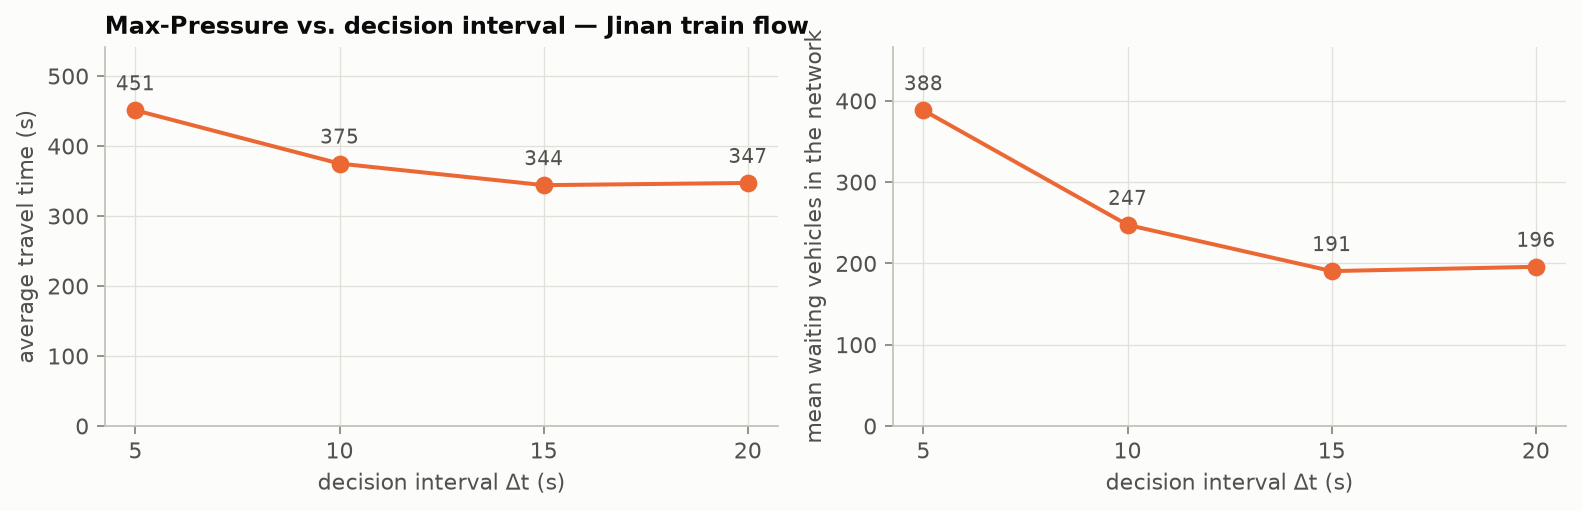
\includegraphics[width=0.62\textwidth]{10_decision_interval.png}
\caption[EDA: Max-Pressure against the decision interval (training flow)]{EDA on the Jinan training flow: Max-Pressure with a decision every $\dt$ seconds.
Average travel time (left) and mean number of waiting vehicles (right) are lowest at
$\dt=15$\,s, the value frozen in the evaluation protocol.}
\label{fig:eda}
\end{figure}

\section{Proposed Model Architecture}
\label{sec:arch}

\Cref{fig:arch} shows the whole system. One network serves all intersections. It encodes
an intersection's observation along with those of its neighbours and scores each phase with
$K$ heads. When the heads disagree too much, the Max-Pressure phase is applied in place of the
learned one.

\begin{figure}[t]
\centering
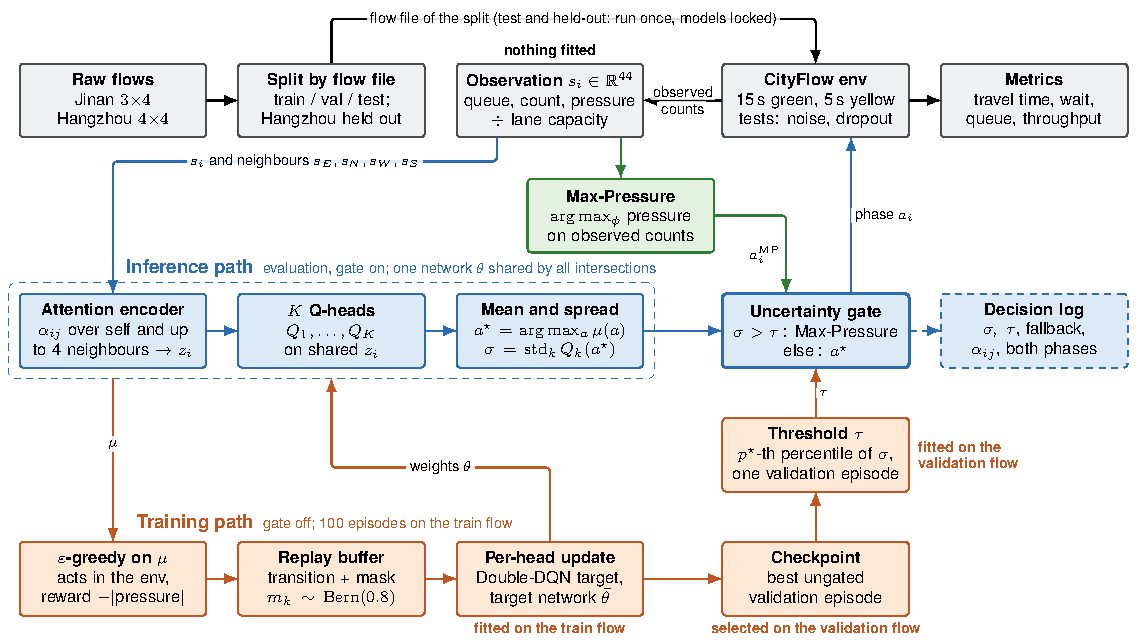
\includegraphics[width=\textwidth]{architecture.pdf}
\caption[\ugmarl{} architecture: data, inference path and training path]{\ugmarl{} architecture in data-flow order. Grey: data and environment. Blue:
inference path with the uncertainty gate. Green: the Max-Pressure fallback. Orange:
training path. Tags mark what is fitted on the training flow and what is fitted or
selected on the validation flow; the observation scaling fits nothing.}
\label{fig:arch}
\end{figure}

\subsection{Decision process}
Every intersection runs on its own clock. When it is ready, it picks the next green phase
$a_i\in\{1,\dots,8\}$ and holds it for $\dt=15$\,s, with 5\,s of transition first whenever the
phase changes. One decision interval therefore lasts $d\in\{15,20\}$\,s, intersections decide
at different moments, and each one faces a semi-Markov decision process. The reward is minus
the absolute pressure at the end of the interval,
\begin{equation}
r_i=-\lvert P_i\rvert,\qquad P_i=\sum_{l\in \mathrm{in}(i)} n_l-\sum_{l\in \mathrm{out}(i)} n_l ,
\label{eq:reward}
\end{equation}
which is the quantity Max-Pressure drives down \citep{varaiya2013max,wei2019presslight}.
The learned policy and its fallback therefore work towards the same goal.

\subsection{Learning target}
The three learned agents (DQN, IDQN and \ugmarl{}) are trained with the Double Q-learning
target, a target network $\bar\theta$, uniform replay and the Huber loss. For a transition
$(s,a,r,s',d)$,
\begin{equation}
y = c\,r+\gamma^{\,d/\dt}\,Q_{\bar\theta}\big(s',\argmax_{a'}Q_\theta(s',a')\big),\qquad
\mathcal L(\theta)=\mathrm{Huber}\big(Q_\theta(s,a)-y\big),
\label{eq:target}
\end{equation}
where the reward scale is fixed at $c=0.01$. Because intervals have different lengths, the
exponent $d/\dt$ discounts by the time that has passed. The episode stops at 3600\,s only
because the simulation does; traffic goes on, so the target always bootstraps.

\subsection{Neighbour attention}
Intersection $i$ sees five slots $j\in\{0{=}\text{self},E,N,W,S\}$, each with a state $s_j$
and a presence flag $m_j$, since an intersection on the border has fewer neighbours. With an
embedding width $d_e$ and a learned slot embedding $p_j$, a single attention layer modelled on
CoLight \citep{wei2019colight} computes
\begin{equation}
e_j=\mathrm{ReLU}(W_e s_j+b_e)+p_j,\qquad
\alpha_{ij}=\frac{m_j\exp\!\big(\langle W_q e_0,\,W_k e_j\rangle/\sqrt{d_e}\big)}
{\sum_{j'}m_{j'}\exp\!\big(\langle W_q e_0,\,W_k e_{j'}\rangle/\sqrt{d_e}\big)},\qquad
z_i=\Big[\,e_0\,\Big\|\,\sum_j\alpha_{ij}W_v e_j\Big].
\label{eq:attention}
\end{equation}
A missing neighbour gets a weight of zero. The same weights therefore handle two, three or
four neighbours, and grids of other sizes. The weight $\alpha_{ij}$ says how much slot $j$
adds to $z_i$. That is an association inside the network and says nothing causal about
how a neighbour affects the action.

\subsection{Q-ensemble and uncertainty}
On top of the shared $z_i$ sit $K$ two-layer heads $Q_1,\dots,Q_K$ (hidden width 128),
each initialised independently. As in Bootstrapped DQN \citep{osband2016deep}, every stored
transition $b$ carries a mask $m_b\in\{0,1\}^K$ with $m_{bk}\sim\mathrm{Bernoulli}(0.8)$. Each
head has its own target $y_{bk}$ from \cref{eq:target}, and the loss on a batch $\mathcal B$ is
\begin{equation}
\mathcal L(\theta)=\frac1K\sum_{k=1}^{K}
\frac{\sum_{b\in\mathcal B}m_{bk}\,\mathrm{Huber}\big(Q_{\theta,k}(s_b,a_b)-y_{bk}\big)}
{\max\big(1,\sum_{b\in\mathcal B}m_{bk}\big)} .
\label{eq:loss}
\end{equation}
The agent acts on the mean of the heads and measures how far they spread at the chosen action,
\begin{equation}
\mu(s,a)=\frac1K\sum_{k}Q_k(s,a),\qquad a^\star=\argmax_a\mu(s,a),\qquad
\sigma(s)=\sqrt{\frac1K\sum_k\big(Q_k(s,a^\star)-\mu(s,a^\star)\big)^2}.
\label{eq:sigma}
\end{equation}
A head predicts an expected return, so the randomness of the traffic is averaged out within
each head. What separates the heads is their initialisation and the experience their masks let
through, which makes $\sigma$ an estimate of epistemic (model) uncertainty. It is a rough
estimate. The heads share an encoder and are correlated, $\sigma$ is measured in Q units and
is not a probability of error, and if all heads extrapolate a state in the same wrong way,
$\sigma$ stays low. With the chosen $K=3$ and $d_e=128$, the network has 157\,720 parameters.

\subsection{Uncertainty gate}
During evaluation, each intersection that is ready to decide applies
\begin{equation}
a_i=\begin{cases}
a_i^{\mathrm{MP}}=\argmax_{\phi}\sum_{m\in\phi}\big(\hat x_{\mathrm{in}(m)}-\hat x_{\mathrm{out}(m)}\big)
& \text{if }\sigma(s_i)>\tau,\\[2pt]
a^\star(s_i) & \text{otherwise,}
\end{cases}
\label{eq:gate}
\end{equation}
where $a_i^{\mathrm{MP}}$ is Max-Pressure computed from the same observed counts $\hat x$ that
the Max-Pressure baseline reads. The gate is off during training and during checkpoint
selection, which means the ablation without the gate uses exactly the same weights. The
threshold $\tau=Q_p(\{\sigma(s_t)\})$ is the $p$-th percentile of the model's $\sigma$ over one
clean validation episode run without the gate. It is computed separately for each trained
model, because the scale of $\sigma$ varies from model to model, but one $p$ serves all seeds.
That $p$ is chosen on validation to minimise mean travel time over the clean flow and four
degraded-detector versions of it. Using the clean flow alone would have chosen never to fall
back, because the learned policy already beats Max-Pressure on it.

\subsection{Safety argument}
\citet{varaiya2013max} proves that Max-Pressure keeps the expected total queue bounded if
queues are points with unlimited storage, turning ratios are known, demand lies strictly inside
the capacity region and the rule runs in every slot on the true queues. When the gate always
fires ($\tau<0$), \ugmarl{} \emph{is} Max-Pressure and the result holds as it stands. For the
mixed policy only a sketch exists. Under any phase choice, the drift of a quadratic queue
function differs from the Max-Pressure drift by a bounded amount per slot. The drift therefore
stays negative if the learned policy acts in few enough slots or if demand sits far enough
inside the capacity region, and a lower $\tau$ moves the system towards the proven case. None
of this covers the controller as it actually runs. Its lanes are finite, it acts every 15\,s on
counts that may be noisy, demand is not guaranteed to stay inside the capacity region, and
a bounded queue does not bound how long one vehicle waits. The mixed policy is therefore not called
provably stable, and its worst case is measured instead (H2).

\section{Algorithm}
\label{sec:algorithm}

\Cref{alg:ugmarl} sets out the full procedure, and each of its lines was checked against
the code.

% Algorithm 1 (ROADMAP 9.6). Checked line by line against the code: checks/algorithm_check.md
\begin{algorithm}[t]
\caption{\ugmarl{} training, tuning and evaluation}
\label{alg:ugmarl}
\footnotesize
\begin{algorithmic}[1]
\Require road network $G$; flows $F_{\mathrm{train}}, F_{\mathrm{val}}, F_{\mathrm{test}}$
(Jinan) and $F_{\mathrm{held}}$ (Hangzhou); grid $H$ of $(K,d_e)$; percentiles $P$; seeds $S$
\Ensure weights $\theta_s$ and threshold $\tau_s$ for every $s\in S$; test and held-out
metrics as mean $\pm$ std and 95\,\% CI
\State Assign whole flow files to train, validation and test; leave $F_{\mathrm{held}}$
unopened; lane capacities $c_l$ from road lengths (nothing is fitted)
\Procedure{Train}{$K, d_e, s$} \Comment{gate off}
  \State initialise $\theta$ with seed $s$; $\bar\theta\gets\theta$; replay $\mathcal D\gets\emptyset$ (100\,000 transitions); $best\gets\infty$
  \For{episode $e=1,\dots,100$ on $F_{\mathrm{train}}$}
    \State $\varepsilon\gets$ linear from 1.0 to 0.05 over the first 30 episodes
    \For{each step, each ready intersection $i$}
      \State $z_i\gets$ attention over $s_i$ and neighbours (\cref{eq:attention}); $\mu\gets$ mean of $Q_1,\dots,Q_K$
      \State $a_i\gets$ random phase with probability $\varepsilon$, else $\argmax_a\mu(s_i,a)$
      \State store $(s,a,r,s',d)$ with mask $m_k\sim\mathrm{Bernoulli}(0.8)$ in $\mathcal D$
      \State every 4 transitions (after the first 2000): one gradient step on \cref{eq:loss}
      \State every 1000 gradient steps: $\bar\theta\gets\theta$
    \EndFor
    \If{$e \bmod 5=0$}
      \State run one greedy episode on $F_{\mathrm{val}}$; if its travel time $<best$, save $\theta$ and update $best$
    \EndIf
  \EndFor
  \State \Return the saved $\theta$
\EndProcedure
\State \textbf{for} $(K,d_e)\in H$: \Call{Train}{$K,d_e,0$};\quad
$(K^\star,d_e^\star)\gets$ smallest $K$, then smallest $d_e$, within 1\,s of the best validation travel time
\State \textbf{for} $s\in S$: $\theta_s\gets$ \Call{Train}{$K^\star,d_e^\star,s$}
\State \textbf{for} $s\in S$: record $\sigma$ of every decision of one clean, ungated episode on
$F_{\mathrm{val}}$; $\tau_s(p)\gets$ $p$-th percentile, $p\in P$
\State $p^\star\gets$ smallest $p\in P$ within 1\,s of the lowest mean travel time of the gated
policy over $S$ and five conditions of $F_{\mathrm{val}}$ (clean, noise 0.1, 0.2, dropout 10, 20\,\%);\quad $\tau_s\gets\tau_s(p^\star)$
\State Lock $(\theta_s,\tau_s)$ with a hash manifest
\For{$s\in S$, each condition of $F_{\mathrm{test}}$ and each flow of $F_{\mathrm{held}}$} \Comment{each episode once}
  \State at every ready intersection apply $a_i\gets a_i^{\mathrm{MP}}$ if $\sigma(s_i)>\tau_s$, else $a^\star(s_i)$ (\cref{eq:gate})
\EndFor
\State Report mean $\pm$ std and 95\,\% CI (Student $t$) over $S$
\end{algorithmic}
\end{algorithm}


\section{Experimental Setup}
\label{sec:setup}

\textbf{Agents.} \Cref{tab:agents} lists the controllers in the comparison and the reason
for including each. They share the environment wrapper, the flows, the episode length, $\dt$
and the seeds. Three ablations take \ugmarl{} apart. $-$gate keeps the same checkpoints and
switches the gate off, $-$attention drops the neighbour input and gets its own threshold from
the same $p$, and $-$ensemble uses $K=1$, which leaves no $\sigma$ and so no gate.

\begin{table}[t]
\centering\small
\caption{Compared controllers and why each is included.}
\label{tab:agents}
\begin{tabular}{lll}
\toprule
Controller & Type & Role in the comparison \\
\midrule
Fixed-Time & conventional & 30\,s green per phase in a fixed cycle; non-adaptive reference \\
Max-Pressure & conventional & pressure rule every $\dt$ \citep{varaiya2013max}; strongest rule baseline and the fallback \\
DQN (shared) & single-agent RL & one network 44--128--128--8 for all intersections, local observation only \\
IDQN & multi-agent RL & one independent network per intersection \\
\ugmarl{} & proposed & neighbour attention, $K$-head ensemble, uncertainty gate (\cref{sec:arch}) \\
\bottomrule
\end{tabular}
\end{table}

\textbf{Training and tuning.} Each learned agent trains for 100 episodes on the training
flow. After every fifth episode it runs one greedy episode on validation, and the checkpoint
with the lowest validation travel time is kept. The search spaces were written into
configuration files before the first tuning run. For DQN and IDQN, 8 of the 36
combinations of learning rate $\{10^{-4},3{\cdot}10^{-4},10^{-3}\}$,
$\gamma\in\{0.8,0.9,0.95\}$, batch size $\{64,128\}$ and exploration decay $\{0.3,0.5\}$ were
sampled and each was trained with seed 0. Both agents ended up with the same winner ($10^{-4}$, 0.8, 64, 0.3).
\ugmarl{} takes these learning settings over unchanged, and only $K\in\{3,5,10\}$ and
$d_e\in\{32,64,128\}$ were searched, as a full grid with seed 0. Three settings came within
the 1\,s tie tolerance of the best (301.1\,s), and the rule set in advance picks the smallest
$K$, which gave $K=3$ and $d_e=128$. The gate percentile was chosen from $\{80,90,95,99\}$. Since
80 and 90 tied within 1\,s, the smaller one, $p^\star=80$, was used.

\textbf{Evaluation.} Every learned agent is trained with seeds 0--4, and seed $s$ is always
evaluated with the model trained on seed $s$. The robustness conditions change the inputs of
\emph{every} controller, Max-Pressure included. They add Gaussian noise with a standard
deviation of 0.1 or 0.2 to the capacity-scaled lane values, drop each lane reading with
probability 10 or 20\,\%, or create a demand surge by duplicating each vehicle with
probability 0.5. Rewards and metrics are always computed on the true state. The evaluation
protocol (splits, $\dt$, reward, metrics, seeds and conditions) was frozen before any learning
agent was trained, and later clarifications carry dates in the project's decision log.

\textbf{Hardware, software, reproducibility.} All final numbers were produced on one laptop
(Intel Core i5-13420H, 12 threads, Ubuntu 24.04) with Python 3.12.3, PyTorch 2.15.0, NumPy
2.5.4 and CityFlow built from a pinned commit. For networks this small the CPU was faster than
the GPU, so training and inference run on the CPU; one training run takes 16--24 minutes. A
configuration file and a seed drive every run, each run is recorded in an experiment log, and
every table and figure can be rebuilt with a documented command.

\chapter{Results and Discussion}
\label{ch:results}

Every number in this chapter comes from the Jinan test flow or the Hangzhou flows. Each
episode was simulated once with the locked models, and the learned agents are reported as the
mean $\pm$ standard deviation over seeds 0--4.

\section{Performance Evaluation Metrics}
\label{sec:metrics}

The \emph{primary metric} is the average travel time over all vehicles in the flow, where a
vehicle still on the road at 3600\,s counts with the time it has spent so far. The secondary metrics are
the average waiting time (speed below 0.1\,m/s), the average queue per incoming lane, the
throughput, meaning the vehicles that left the network, and, as the safety metric, the longest
wait of any single vehicle. The fallback rate is the share of \ugmarl{} decisions that
Max-Pressure made. Efficiency is measured as decision latency, training time and parameter
count.

Each metric comes with a 95\,\% confidence interval from Student's $t$ distribution with
four degrees of freedom. A difference is \emph{clear} when the two intervals do not
overlap, or, against a deterministic rule controller, when the whole interval sits on one side
of its value. Otherwise the two are \emph{level}. A model's \emph{regret} in a condition is
its mean travel time minus the lowest mean of the five controllers in that condition. The
rules for judging the hypotheses were written down before the test flow was opened. For H2,
the gated model has to beat the same checkpoints without the gate on three counts: (i) a lower
maximum wait on clean data, (ii) a lower maximum wait at noise 0.2, and (iii) a smaller rise
in travel time from clean data to noise 0.2.

\section{Experimental Results}
\label{sec:results}

\begin{table}[t]
\centering\footnotesize
\setlength{\tabcolsep}{4.2pt}
\caption[Main comparison on the Jinan test flow]{Main comparison on the Jinan test flow with clean detectors (5 seeds; rule
controllers are deterministic). Val.\ = validation travel time, used for selection and
therefore optimistic; Queue in vehicles per lane; Thr.\ = throughput in vehicles; Train =
minutes per run. Bold: lowest test travel time.}
\label{tab:main}
% Generated by scripts/report_tables.py from docs/results/*.csv -- do not edit.
\begin{tabular}{lrrcrrrrrr}
\toprule
Model & Val.\ (s) & Test (s) & 95\,\% CI & Wait (s) & Queue & Thr. & Max wait (s) & Train & Params \\
\midrule
Fixed-Time & 434.8 & 462.2 & -- & 210.1 & 2.19 & 4617 & 1417 & -- & 0 \\
Max-Pressure & 326.1 & 320.8 & -- & 87.9 & 0.95 & 4950 & 1219 & -- & 0 \\
\midrule
DQN (shared) & 299.8 $\pm$ 1.0 & \textbf{292.2 $\pm$ 0.6} & [291.4, 293.0] & 57.0 & 0.63 & 5007 & 772 $\pm$ 126 & 23.6 & 23\,304 \\
IDQN & 312.7 $\pm$ 2.5 & 307.9 $\pm$ 1.4 & [306.1, 309.7] & 72.3 & 0.79 & 4980 & 749 $\pm$ 85 & 22.2 & 279\,648 \\
\midrule
UG-MARL (proposed) & 302.3 $\pm$ 1.1 & 295.4 $\pm$ 1.1 & [294.1, 296.8] & 60.5 & 0.66 & 4996 & 896 $\pm$ 169 & 18.2 & 157\,720 \\
\bottomrule
\end{tabular}

\end{table}

\Cref{tab:main} has the main comparison. \ugmarl{} reaches \res{tt}{ugmarl}{clean}\,s, and
its whole interval lies below Max-Pressure (\res{tt}{max_pressure}{clean}\,s) and below the
interval of IDQN (\res{tt}{idqn}{clean}\,s), so \textbf{H1 is supported}. That makes it 25\,s
(8\,\%) faster than the best rule controller and 12.5\,s faster than the standard multi-agent
learner. Waiting time, queue length and throughput put the controllers in the same order.

On clean data the best controller is the single shared DQN (\res{tt}{dqn}{clean}\,s).
\ugmarl{} trails it by \res{regret}{ugmarl}{clean}\,s (1.1\,\%) and the intervals do not
overlap. None of the hypotheses was about this comparison, but it is a loss and is reported
as one. The maximum wait of \ugmarl{} (\res{maxw}{ugmarl}{clean}\,s) is lower than that of
Max-Pressure (\res{maxw}{max_pressure}{clean}\,s), which meets the minimum outcome set in
advance. Against DQN and IDQN it is level, since the intervals overlap.

\section{Comparison with Existing Models}
\label{sec:comparison}

\begin{table}[t]
\centering\footnotesize
\setlength{\tabcolsep}{3.4pt}
\caption[Travel time under six test conditions and worst-case regret]{Average travel time (s) on the Jinan test flow under six conditions, mean $\pm$
std over 5 seeds. Regret = largest gap to the best of the five controllers over the
conditions. Bold: best of the five controllers in the column.}
\label{tab:robust}
% Generated by scripts/report_tables.py from docs/results/*.csv -- do not edit.
\begin{tabular}{lrrrrrrr}
\toprule
Model & Clean & Noise 0.1 & Noise 0.2 & Dropout 10\,\% & Dropout 20\,\% & Surge $\times$1.5 & Regret \\
\midrule
Fixed-Time & 462.2 & 462.2 & 462.2 & 462.2 & 462.2 & 661.4 $\pm$ 4.2 & 288.4 \\
Max-Pressure & 320.8 & \textbf{366.9 $\pm$ 1.7} & \textbf{413.7 $\pm$ 4.0} & 317.8 $\pm$ 0.8 & 317.2 $\pm$ 2.1 & 435.2 $\pm$ 4.3 & 62.2 \\
DQN (shared) & \textbf{292.2 $\pm$ 0.6} & 569.8 $\pm$ 32.0 & 828.2 $\pm$ 36.3 & \textbf{298.3 $\pm$ 0.8} & \textbf{304.8 $\pm$ 1.1} & \textbf{373.0 $\pm$ 4.6} & 414.6 \\
IDQN & 307.9 $\pm$ 1.4 & 543.3 $\pm$ 54.2 & 758.9 $\pm$ 33.6 & 313.4 $\pm$ 1.4 & 322.3 $\pm$ 1.1 & 455.3 $\pm$ 71.5 & 345.2 \\
UG-MARL (proposed) & 295.4 $\pm$ 1.1 & 370.4 $\pm$ 6.8 & 420.5 $\pm$ 7.4 & 299.8 $\pm$ 1.8 & 305.1 $\pm$ 3.2 & 375.0 $\pm$ 4.9 & \textbf{6.8} \\
\midrule
UG-MARL $-$gate & 295.0 $\pm$ 1.0 & 597.7 $\pm$ 53.5 & 870.2 $\pm$ 45.0 & 300.1 $\pm$ 2.3 & 305.4 $\pm$ 4.6 & 376.4 $\pm$ 5.4 & 456.6 \\
\bottomrule
\end{tabular}

\end{table}

The comparison covers the four baselines run in this project, on the same flows, seeds and
settings. Published travel times for Jinan and Hangzhou do not appear in the tables, because
those studies used other decision intervals and transition times.

\Cref{tab:robust} adds degraded detectors and a demand surge, and each baseline does
badly in at least one of these conditions. DQN is best with clean detectors, with dropped
readings and under the surge. With detector noise of 0.2, though, DQN and IDQN climb to
\res{tt}{dqn}{noise0.2} and \res{tt}{idqn}{noise0.2}\,s, well above even Fixed-Time.
Max-Pressure shows the opposite pattern. It is best under noise and 12--62\,s behind the best
controller in the other conditions. In each condition \ugmarl{} stays close to whichever of the
two does better. At noise 0.2 it holds \res{tt}{ugmarl}{noise0.2}\,s, level with Max-Pressure
(\res{tt}{max_pressure}{noise0.2}\,s), and under dropout and the surge it is level with DQN.
Over the six conditions its largest regret is \res{regret}{ugmarl}{worst}\,s. For Max-Pressure
it is \res{regret}{max_pressure}{worst}\,s, for IDQN \res{regret}{idqn}{worst}\,s and for DQN
\res{regret}{dqn}{worst}\,s. \ugmarl{} wins none of the conditions, and it is never far
behind the winner.

\textbf{H2 is supported} under the three-part rule. With the gate, the maximum wait is
\res{maxw}{ugmarl}{clean} against \res{maxw}{ugmarl-nogate}{clean}\,s on clean data and
\res{maxw}{ugmarl}{noise0.2} against \res{maxw}{ugmarl-nogate}{noise0.2}\,s at noise 0.2,
and the travel time goes up by \res{dtt}{ugmarl}{noise0.2} instead of
\res{dtt}{ugmarl-nogate}{noise0.2}\,s. Parts (ii) and (iii) are clear, with paired intervals
of $[-2306,-1320]$\,s and $[-512,-388]$\,s. Part (i) falls inside seed noise (paired interval
$[-382,353]$\,s). One vehicle sets the maximum wait, and it ranges from 631 to 1052\,s across
the seeds of \ugmarl{}, so on clean data the gate makes no measurable difference.

\section{Graphical Analysis}
\label{sec:graphs}

\begin{figure}[t]
\centering
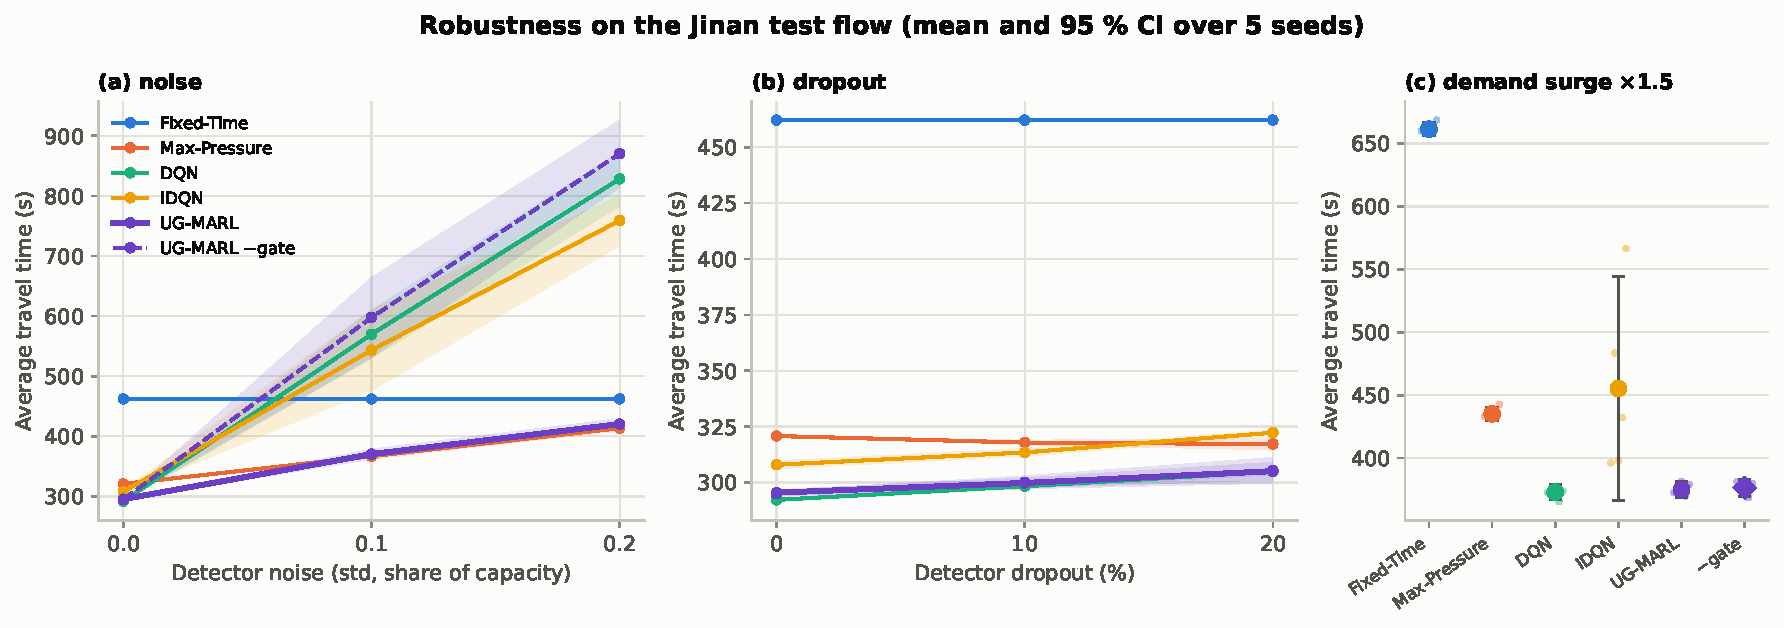
\includegraphics[width=\textwidth]{robustness_degradation.pdf}
\caption[Robustness to detector noise, dropout and demand surge]{Robustness on the Jinan test flow (mean and 95\,\% CI over 5 seeds). (a) Under
detector noise the ungated learned controllers lose 450--575\,s, while \ugmarl{} follows
Max-Pressure. (b) Dropout costs every controller less than 15\,s. (c) Under the demand surge
\ugmarl{} stays with DQN; IDQN becomes unstable across seeds.}
\label{fig:robust}
\end{figure}

\Cref{fig:robust} plots travel time against the three kinds of disturbance. The curves for
\ugmarl{} with and without the gate start at the same point and part as soon as noise is
added. Without the gate the model collapses under noise, and with it the model loses only as
much as Max-Pressure does. Dropout hardly matters, because a lost reading is set to zero and
looks like an empty lane, a state the agents saw in training.

\begin{figure}[t]
\centering
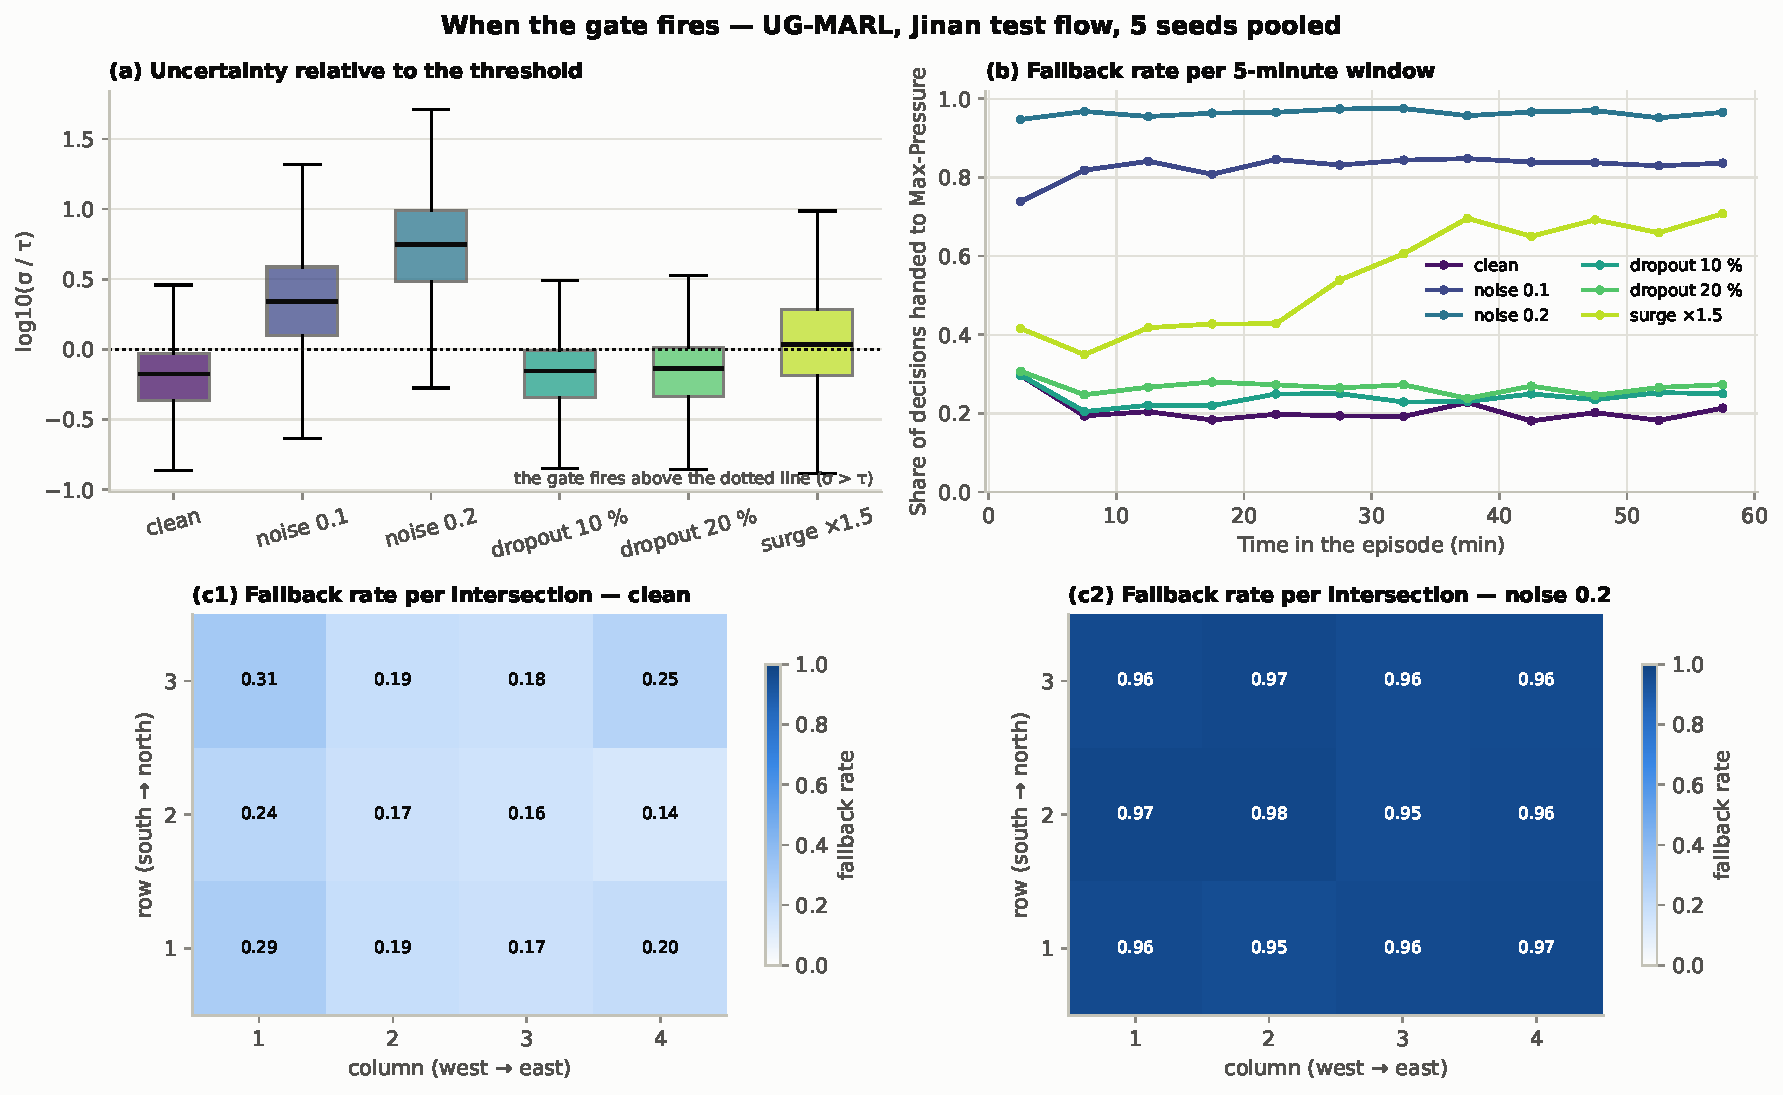
\includegraphics[width=0.68\textwidth]{gate_firing.pdf}
\caption[When and where the uncertainty gate fires]{When the gate fires (\ugmarl{}, Jinan test flow, 5 seeds pooled). (a) $\sigma$
relative to the threshold: the median is below $\tau$ on clean data and under dropout,
about $2\tau$ at noise 0.1 and $6\tau$ at noise 0.2. (b) Fallback rate over the hour: constant
except under the surge, where it rises from about 40 to 70\,\%. (c) Fallback rate per
intersection: 14--31\,\% on clean data, 95--98\,\% at noise 0.2.}
\label{fig:gate}
\end{figure}

\Cref{fig:gate} explains the pattern. The uncertainty $\sigma$ of \cref{eq:sigma} goes up
with detector noise, and the gate passes \res{fb}{ugmarl}{noise0.1}\,\% of decisions to
Max-Pressure at noise 0.1 and \res{fb}{ugmarl}{noise0.2}\,\% at noise 0.2, compared with
\res{fb}{ugmarl}{clean}\,\% on clean data. Dropout leaves it almost unchanged
(\res{fb}{ugmarl}{drop0.1} and \res{fb}{ugmarl}{drop0.2}\,\%). The detectors are clean during
the surge, yet $\sigma$ grows with the queues, and the fallback rate climbs through the hour
to an average of \res{fb}{ugmarl}{surge1.5}\,\%. In short, $\sigma$ responds to any input that
looks unlike the training data, whatever caused it.

\section{Discussion of Findings}
\label{sec:discussion}

\subsection{Ablation}
\begin{table}[t]
\centering\footnotesize
\setlength{\tabcolsep}{2.6pt}
\caption[Ablation of gate, attention and ensemble]{Ablation on the Jinan test flow (5 seeds). Travel time in seconds for three
conditions; $\Delta$ = difference to the full model on clean data; maximum wait in seconds;
FB = fallback rate on clean data.}
\label{tab:ablation}
% Generated by scripts/report_tables.py from docs/results/*.csv -- do not edit.
\begin{tabular}{lrrrrrrrr}
\toprule
Variant & Clean (s) & $\Delta$ (s) & Noise 0.2 (s) & Surge (s) & Max wait, clean & Max wait, noise 0.2 & FB (\%) & Params \\
\midrule
UG-MARL (full) & 295.4 $\pm$ 1.1 & -- & 420.5 $\pm$ 7.4 & 375.0 $\pm$ 4.9 & 896 $\pm$ 169 & 1493 $\pm$ 220 & 21 & 157\,720 \\
UG-MARL $-$gate & 295.0 $\pm$ 1.0 & $-$0.4 & 870.2 $\pm$ 45.0 & 376.4 $\pm$ 5.4 & 910 $\pm$ 190 & 3306 $\pm$ 323 & 0 & 157\,720 \\
UG-MARL $-$attention & 294.2 $\pm$ 1.1 & $-$1.2 & 419.3 $\pm$ 3.1 & 376.3 $\pm$ 2.8 & 876 $\pm$ 120 & 1410 $\pm$ 202 & 21 & 59\,032 \\
UG-MARL $-$ensemble & 297.3 $\pm$ 1.5 & $+$1.9 & 864.9 $\pm$ 134.8 & 395.1 $\pm$ 40.1 & 740 $\pm$ 238 & 3279 $\pm$ 259 & 0 & 89\,864 \\
\bottomrule
\end{tabular}

\end{table}

\Cref{tab:ablation} takes the three components out one at a time. Removing the
\emph{gate} changes nothing measurable on clean data (paired difference $0.4\pm0.9$\,s) and
costs 450\,s at noise 0.2. Without the \emph{ensemble} ($K=1$) there is no uncertainty
estimate and hence no gate, and the model fails under noise just like the other ungated
learners; on clean data it is 1.9\,s behind the full model, with overlapping intervals.
Without \emph{attention}, the model reaches \res{tt}{ugmarl-noattn}{clean}\,s against
\res{tt}{ugmarl}{clean}\,s for the full model, with overlapping intervals and 63\,\% fewer
parameters. \textbf{H3 is not supported}. Neighbour attention did not lower travel time in
any of the six conditions or on Hangzhou.

\subsection{Generalisation}
\begin{table}[t]
\centering\footnotesize
\setlength{\tabcolsep}{3.6pt}
\caption[Zero-shot generalisation to Hangzhou]{Zero-shot evaluation on Hangzhou ($4\times4$, three flows, 5 seeds): average
travel time in seconds. Models were trained on the Jinan training flow and thresholds come
from Jinan validation. ``All flows'' averages the flows per seed; maximum wait and fallback
rate (FB) are over all flows. Bold: lowest travel time.}
\label{tab:heldout}
% Generated by scripts/report_tables.py from docs/results/*.csv -- do not edit.
\begin{tabular}{lrrrrcrr}
\toprule
Model & Flow A & Flow B & Flow C & All flows (s) & 95\,\% CI & Max wait (s) & FB (\%) \\
\midrule
Fixed-Time & 590.5 & 841.7 & 570.2 & 667.5 & -- & 1756 & 0 \\
Max-Pressure & 360.7 & 500.0 & 434.7 & 431.8 & -- & 2734 & 0 \\
\midrule
DQN (shared) & 343.4 $\pm$ 2.1 & 478.7 $\pm$ 22.7 & 409.1 $\pm$ 4.9 & 410.4 $\pm$ 7.1 & [401.6, 419.3] & 1660 $\pm$ 272 & 0 \\
IDQN & \multicolumn{7}{c}{not transferable (one network per Jinan intersection)} \\
\midrule
UG-MARL (proposed) & 347.3 $\pm$ 3.5 & 466.4 $\pm$ 8.5 & 416.3 $\pm$ 2.6 & 410.0 $\pm$ 2.9 & [406.4, 413.6] & 2262 $\pm$ 206 & 34 \\
UG-MARL $-$gate & 348.9 $\pm$ 4.3 & 491.7 $\pm$ 35.6 & 419.8 $\pm$ 10.1 & 420.1 $\pm$ 14.6 & [402.0, 438.2] & 1939 $\pm$ 375 & 0 \\
UG-MARL $-$attention & 341.5 $\pm$ 0.7 & 460.2 $\pm$ 5.1 & 409.6 $\pm$ 1.9 & \textbf{403.8 $\pm$ 1.2} & [402.3, 405.2] & 2146 $\pm$ 153 & 37 \\
UG-MARL $-$ensemble & 351.7 $\pm$ 2.9 & 493.7 $\pm$ 39.2 & 425.7 $\pm$ 8.9 & 423.7 $\pm$ 14.9 & [405.2, 442.2] & 1696 $\pm$ 237 & 0 \\
\bottomrule
\end{tabular}

\end{table}

\Cref{tab:heldout} shows the zero-shot results on a city and a grid size that played no
part in training or tuning. The ranking is the same as on Jinan: learned controllers first,
then Max-Pressure, then Fixed-Time. \ugmarl{} (\res{tt}{ugmarl}{hz-all}\,s) is level with DQN
(\res{tt}{dqn}{hz-all}\,s) and 22\,s ahead of Max-Pressure. Its gate fires more often here
than on Jinan (\res{fb}{ugmarl}{hz-all}\,\% against \res{fb}{ugmarl}{clean}\,\%), and it
removes most of the spread between seeds that the ungated model shows
($\pm$\res{ttsd}{ugmarl}{hz-all} against $\pm$\res{ttsd}{ugmarl-nogate}{hz-all}\,s). IDQN
cannot be moved to Hangzhou at all, since it keeps one network for each Jinan intersection.

\subsection{Error analysis}
The saved logs were split by intersection, by 10-minute window and by route.
\begin{itemize}
\item \emph{Where \ugmarl{} wins.} Compared with Max-Pressure on clean data, vehicles wait
17--40\,\% less at each of the 12 intersections. The gain grows with route length, from 12\,s
for trips through one intersection to 37\,s for trips through four or more.
\item \emph{Where it loses.} The 3.2\,s deficit to DQN is spread out. Waiting is higher at
every intersection (by up to 12\,\%), in every time window and for every route length. The
gate is not to blame, because the same checkpoints without it are level with the gated model.
All four \ugmarl{} variants trail DQN, so the gap comes either from the network family or
from its learning settings, which were tuned for DQN and reused. The available runs cannot tell
these two apart.
\item \emph{A failure the metrics hide.} At noise 0.2 the ungated learned controllers keep
584--795 of the 5494 vehicles (11--14\,\%) out of the network for the whole hour, because the
entry roads stay jammed. \ugmarl{} and Max-Pressure keep none out. The waiting-time metrics
only count waiting \emph{inside} the network, so the maximum wait of about 3300\,s reported
for these models understates how badly they do.
\item \emph{What the gate costs under a surge.} During the surge the gate leaves travel time
unchanged (\res{tt}{ugmarl}{surge1.5} against \res{tt}{ugmarl-nogate}{surge1.5}\,s) but pushes
the maximum wait up to \res{maxw}{ugmarl}{surge1.5}\,s, compared with
\res{maxw}{ugmarl-nogate}{surge1.5}\,s without the gate and \res{maxw}{dqn}{surge1.5}\,s for
DQN. Max-Pressure alone reaches \res{maxw}{max_pressure}{surge1.5}\,s. Once the gate hands it
most of the decisions, \ugmarl{} picks up its habit of leaving single vehicles waiting a long
time. The most congested Hangzhou flow shows the same thing.
\item \emph{Stability of decisions.} \ugmarl{} switches back to the previous phase after one
interval in 21.5\,\% of its decisions, against 20.2\,\% for DQN and 20.3\,\% for
Max-Pressure, so the gate does not add switching.
\end{itemize}

\subsection{Explainability}
For each decision the system logs $\sigma$, $\tau$, whether the gate fired, the learned
phase, the Max-Pressure phase and the attention weights. These are associations, and two
checks on validation data show how far they can be read. The first is that $\sigma$ has almost
no correlation with the temporal-difference error (Spearman $\rho\approx0.03$). It flags
unfamiliar inputs and says little about whether an action is wrong. The second check swaps
out one neighbour's observation. Swapping the neighbour with the highest attention weight
moves the Q-value more than swapping the one with the lowest (0.0061 against 0.0022, paired
interval $[0.0011, 0.0066]$), so the weights do rank the neighbours' influence. Doing the same
to the intersection's own observation moves Q by 0.0415, about seven times as much, and the own
slot gets a mean weight of 0.82. Decisions are therefore made almost entirely from local
information, which fits the H3 result. One likely reason is that the movement pressures in
\cref{eq:state} already include the downstream lanes that a neighbour would report.

\subsection{Threshold and cost}
A validation sweep run after the final evaluation shows that the exact threshold matters
little. Every percentile from 50 to 90 lands within 5\,s of the chosen $p^\star=80$. $p=70$
would have been 1.5\,s better, so the bottom of the original grid was binding, but the choice
was left as it was. One joint decision for all 12 intersections takes 0.81\,ms with \ugmarl{},
0.22\,ms with DQN and 0.14\,ms with Max-Pressure on a single CPU thread, far inside the 15\,s
decision interval.

\chapter{Conclusion and Future Scope}
\label{ch:conclusion}

\section{Key Findings}

This project compared conventional, single-agent and multi-agent signal controllers on real
traffic flows and built \ugmarl{}, a multi-agent controller that estimates its own uncertainty and
lets Max-Pressure make the decision whenever that uncertainty is high.
\begin{itemize}
\item \textbf{H1, performance: supported.} On the test flow \ugmarl{} averages
\res{tt}{ugmarl}{clean}\,s of travel time, clearly below Max-Pressure
(\res{tt}{max_pressure}{clean}\,s) and IDQN (\res{tt}{idqn}{clean}\,s), and
\res{regret}{ugmarl}{clean}\,s behind the single shared DQN.
\item \textbf{H2, safety: supported}, with one of its three parts undecided. At detector
noise 0.2 the gate holds travel time at \res{tt}{ugmarl}{noise0.2}\,s, where the same model
without it reaches \res{tt}{ugmarl-nogate}{noise0.2}\,s, and keeps the maximum wait at
\res{maxw}{ugmarl}{noise0.2} instead of \res{maxw}{ugmarl-nogate}{noise0.2}\,s. On clean data
the gate makes no measurable difference.
\item \textbf{H3, coordination: not supported.} Neighbour attention did not reduce travel
time, and the model without it does as well with 63\,\% fewer parameters.
\item \textbf{Reliability across conditions.} Each baseline has a condition where it does
badly: the learned ones under detector noise, Max-Pressure on clean data and in the surge.
The largest regret of \ugmarl{} over the six conditions is \res{regret}{ugmarl}{worst}\,s,
against \res{regret}{max_pressure}{worst}--\res{regret}{dqn}{worst}\,s for the baselines, and
on an unseen city it performs at the level of DQN.
\item \textbf{What the uncertainty measures.} $\sigma$ rises for inputs that look unlike the
training data. This is why the gate helps under detector noise. It is also why the gate fires
during a demand surge, where it makes the longest wait worse.
\end{itemize}

\section{Limitations}

\textbf{Evidence.} The study rests on five seeds and one test flow per city. The confidence
intervals capture the randomness of training and say nothing about how demand varies from day
to day. Differences of a few seconds, such as the gap to DQN or the threshold sweep, are close
to what the study can resolve. Because the validation flow was used again and again to pick
checkpoints, the architecture and the threshold, the validation numbers are optimistic. The
cause of the gap to DQN has not been isolated.

\textbf{Method.} Three heads on a shared encoder produce the uncertainty estimate. The signal is
coarse: it cannot tell faulty detectors from heavy demand, and it barely correlates with the
learning error. The gated policy comes with no stability guarantee, and the fallback puts no
bound on how long one vehicle waits. Vehicles that never get into the network are missing from
the waiting-time metrics. Only Gaussian noise and randomly lost readings were tested, not
detectors that are stuck, biased or delayed.

\textbf{Scope.} Both cities are regular grids with a single vehicle class and no pedestrians,
buses or incidents, and both are simulated in CityFlow. With a 15\,s decision interval, the
absolute numbers cannot be compared with studies that use 10\,s. Only two rule baselines
were run.

\textbf{Ethics and deployment.} The data comes without a stated licence, so it is used only for
coursework and is not redistributed. The trips are anonymous and carry no identifiers, so no
personal data is processed. Fairness between road users was examined through waiting per
approach. The learned controllers share waiting evenly across the four approaches (22--29\,\%
each), and the longest unbroken queue on one approach lasts 849\,s under \ugmarl{} against
1275\,s under Max-Pressure. Individual vehicles can still wait a very long time when demand is
heavy. The controller has only been run in simulation and has no safety certification, and the
gap between the simulator and real roads is unknown. Putting it on a real road would need fixed
limits on red time, pedestrian phases and supervision by traffic engineers.

\section{Future Research Directions}

The results suggest four next steps. (1) A fallback with a hard cap on the red time of each
movement would bound the worst case of a single vehicle by design. (2) The gate needs a signal
that tells unreliable inputs apart from heavy but correctly measured demand, for instance by
adding a queue-based trigger or randomised prior functions to the ensemble. (3) Filtering the detector
readings before they reach the fallback, since without filtering none of the controllers here
beats Max-Pressure under noise. (4) Tuning the learning settings of \ugmarl{} on their own and
running more seeds, to find out whether the gap to DQN comes from the architecture. Tests on
irregular networks and with realistic detector faults would show how far these findings hold.


\phantomsection
\addcontentsline{toc}{chapter}{References}
\begingroup
\footnotesize
\setlength{\bibsep}{0.5pt plus 0.3pt}
\bibliographystyle{IEEEtranN}
\bibliography{references}
\endgroup

\appendix
\chapter{Appendix}
\label{ch:appendix}

\section{Code, Poster and Data}
\label{sec:app-links}

\begin{itemize}
\item Code: \url{https://github.com/Saad-Manda/PBL-Agentic-AI}. The repository has the
\texttt{trafficrl} package, the scripts and configuration files for every run, the result
CSVs in \texttt{docs/results/}, and the SHA-256 hashes of the final checkpoints in
\texttt{models/manifest.json}.
\item Poster: \posterlink
\item Data: the Jinan and Hangzhou flows of the CoLight repository \cite{wei2019colight},
\url{https://github.com/wingsweihua/colight}, commit \texttt{04440b7}. The split is defined in
\texttt{data/processed/splits.json} (\cref{sec:dataset}).
\end{itemize}

\section{Learning Curves}
\label{sec:app-curves}

\begin{figure}[ht]
\centering
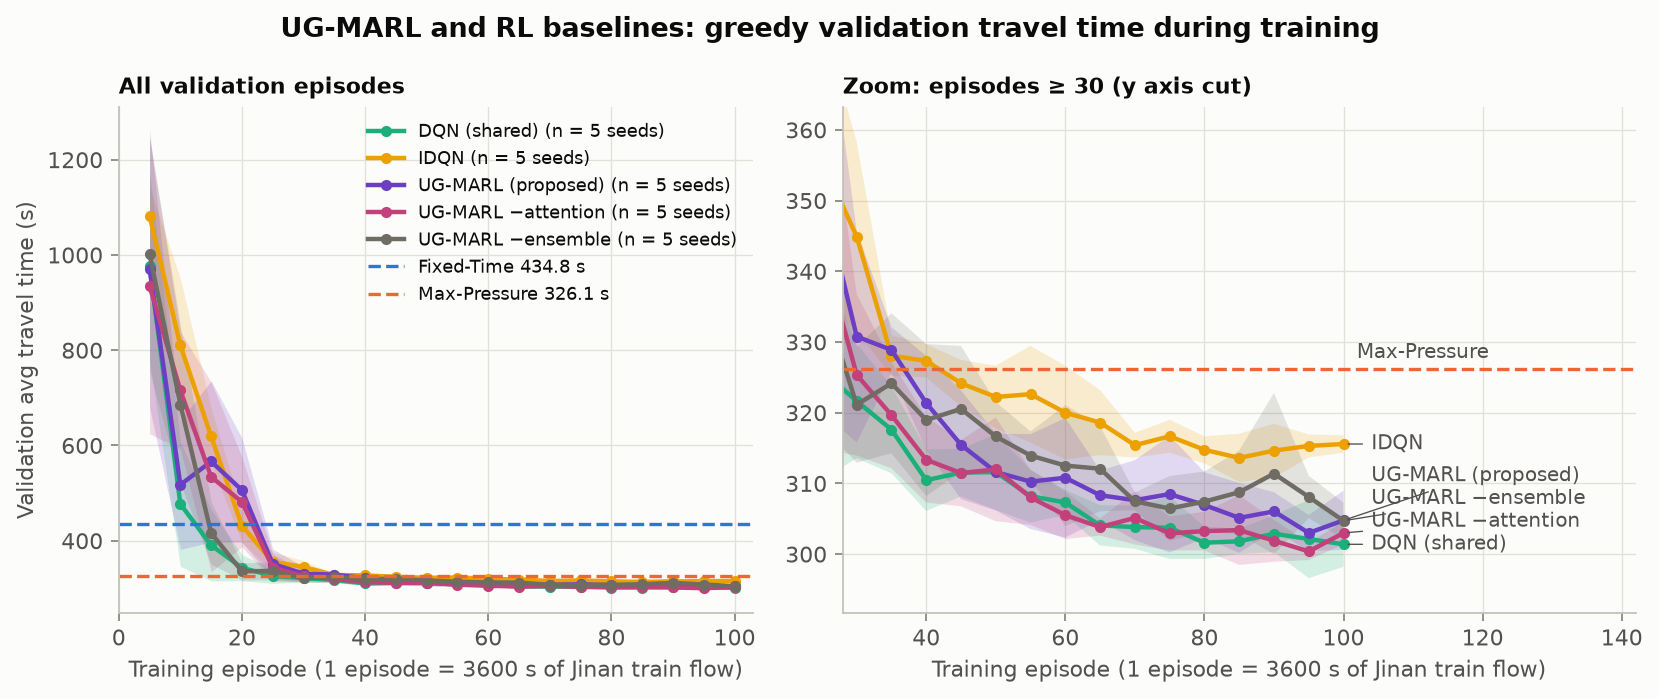
\includegraphics[width=\textwidth]{learning_curves_phase6.png}
\caption[Validation travel time during training]{Average travel time (s) of the greedy
policy on the Jinan validation flow, evaluated every 5 training episodes (mean over seeds
0--4, band = 95\,\% CI). Dashed: Fixed-Time and Max-Pressure on the same flow. Right: episodes
$\geq 30$ with the $y$ axis cut.}
\label{fig:learning-curves}
\end{figure}

Every learned controller drops below Max-Pressure between episodes 25 and 45 of its 100
training episodes (\cref{fig:learning-curves}). Over the last 30 episodes the curves move by
about as much as the seeds differ from each other, which supports the training length set in
\cref{sec:setup}. The checkpoint kept for
each seed is the evaluation with the lowest validation travel time. IDQN stays about 10\,s
above the other learners, which fits its design: each of its twelve networks learns from one
intersection's data only.

    
\end{document}
